\documentclass[12pt,]{article}
\usepackage[left=1in,top=1in,right=1in,bottom=1in]{geometry}
\newcommand*{\authorfont}{\fontfamily{phv}\selectfont}
\usepackage[]{mathpazo}


  \usepackage[T1]{fontenc}
  \usepackage[utf8]{inputenc}




\usepackage{abstract}
\renewcommand{\abstractname}{}    % clear the title
\renewcommand{\absnamepos}{empty} % originally center

\renewenvironment{abstract}
 {{%
    \setlength{\leftmargin}{0mm}
    \setlength{\rightmargin}{\leftmargin}%
  }%
  \relax}
 {\endlist}

\makeatletter
\def\@maketitle{%
  \newpage
%  \null
%  \vskip 2em%
%  \begin{center}%
  \let \footnote \thanks
    {\fontsize{18}{20}\selectfont\raggedright  \setlength{\parindent}{0pt} \@title \par}%
}
%\fi
\makeatother




\setcounter{secnumdepth}{0}

\usepackage{longtable,booktabs}

\usepackage{graphicx,grffile}
\makeatletter
\def\maxwidth{\ifdim\Gin@nat@width>\linewidth\linewidth\else\Gin@nat@width\fi}
\def\maxheight{\ifdim\Gin@nat@height>\textheight\textheight\else\Gin@nat@height\fi}
\makeatother
% Scale images if necessary, so that they will not overflow the page
% margins by default, and it is still possible to overwrite the defaults
% using explicit options in \includegraphics[width, height, ...]{}
\setkeys{Gin}{width=\maxwidth,height=\maxheight,keepaspectratio}


\title{Political Donor Motivations and Public Support of Policies: A Time
Series-Analysis  }



\author{\Large \vspace{0.05in} \newline\normalsize\emph{}  }


\date{}

\usepackage{titlesec}

\titleformat*{\section}{\normalsize\bfseries}
\titleformat*{\subsection}{\normalsize\itshape}
\titleformat*{\subsubsection}{\normalsize\itshape}
\titleformat*{\paragraph}{\normalsize\itshape}
\titleformat*{\subparagraph}{\normalsize\itshape}





\newtheorem{hypothesis}{Hypothesis}
\usepackage{setspace}


% set default figure placement to htbp
\makeatletter
\def\fps@figure{htbp}
\makeatother

\usepackage{graphicx}
\usepackage{booktabs}
\usepackage{longtable}
\usepackage{array}
\usepackage{multirow}
\usepackage{wrapfig}
\usepackage{float}
\usepackage{colortbl}
\usepackage{pdflscape}
\usepackage{tabu}
\usepackage{threeparttable}
\usepackage{threeparttablex}
\usepackage[normalem]{ulem}
\usepackage{makecell}
\usepackage{xcolor}

% move the hyperref stuff down here, after header-includes, to allow for - \usepackage{hyperref}

\makeatletter
\@ifpackageloaded{hyperref}{}{%
\ifxetex
  \PassOptionsToPackage{hyphens}{url}\usepackage[setpagesize=false, % page size defined by xetex
              unicode=false, % unicode breaks when used with xetex
              xetex]{hyperref}
\else
  \PassOptionsToPackage{hyphens}{url}\usepackage[draft,unicode=true]{hyperref}
\fi
}

\@ifpackageloaded{color}{
    \PassOptionsToPackage{usenames,dvipsnames}{color}
}{%
    \usepackage[usenames,dvipsnames]{color}
}
\makeatother
\hypersetup{breaklinks=true,
            bookmarks=true,
            pdfauthor={ ()},
             pdfkeywords = {},  
            pdftitle={Political Donor Motivations and Public Support of Policies: A Time
Series-Analysis},
            colorlinks=true,
            citecolor=blue,
            urlcolor=blue,
            linkcolor=magenta,
            pdfborder={0 0 0}}
\urlstyle{same}  % don't use monospace font for urls

% Add an option for endnotes. -----


% add tightlist ----------
\providecommand{\tightlist}{%
\setlength{\itemsep}{0pt}\setlength{\parskip}{0pt}}

% add some other packages ----------

% \usepackage{multicol}
% This should regulate where figures float
% See: https://tex.stackexchange.com/questions/2275/keeping-tables-figures-close-to-where-they-are-mentioned
\usepackage[section]{placeins}


\begin{document}
	
% \pagenumbering{arabic}% resets `page` counter to 1 
%
% \maketitle

{% \usefont{T1}{pnc}{m}{n}
\setlength{\parindent}{0pt}
\thispagestyle{plain}
{\fontsize{18}{20}\selectfont\raggedright 
\maketitle  % title \par  

}

{
   \vskip 13.5pt\relax \normalsize\fontsize{11}{12} 
\textbf{\authorfont } \hskip 15pt \emph{\small }   

}

}








\begin{abstract}

    \hbox{\vrule height .2pt width 39.14pc}

    \vskip 8.5pt % \small 

\noindent The two predominant theories of political donor motivations are the
access-oriented model and the consumption model. This paper combines
political donation records and social media posts from politicians to
test whether either behavior is observed. In the access-oriented model,
individual political donors and political action committees (PACs) are
assumed to contribute to campaigns in an effort to acquire access and
influence politicians into supporting specific policy issues. In this
study, the access-oriented model of donors predicts that donations from
specific groups of donors will precede public support of certain
policies. The consumption model of donors views political contributions
as being an extension of voting along a participatory spectrum, and that
donors support candidates who they already know support policy issues
that the donors care about or are ideologically motivated. In this
research, the consumption model predicts that donations from various
groups of donors will lag in response to public support of certain
policy issues. Historically, these two models have treated political
donors as all having the same motivations. More recent studies in
campaign finance have found that both motivational models can exist in
different groups of donors. However, these studies categorize groups of
donors in broad strokes, generally as either small-dollar donors and
large-dollar donors as well as PACs. This paper statistically derives
coalitions of similar donors and tests the competing models of political
donor motivations on these more granular groups of donors who support
similar candidates.


    \hbox{\vrule height .2pt width 39.14pc}


\end{abstract}


\vskip -8.5pt


 % removetitleabstract

\noindent \doublespacing 

\newpage

\hypertarget{introduction}{%
\section{Introduction}\label{introduction}}

The amount of money raised and spent by political campaigns in the
United States continues to rise with each election cycle (Goldmacher
2020). However, the explanations of the motivations of political donors,
the psychological reasons why political donors decide to make a
contribution, remain divided. The predominant theories of political
donor motivation fall into two broad categories, the access-oriented
model or the consumption model. In the access-oriented model,
contributions are given in exchange for access and political favors that
presumably materialize in altered government policy. The consumption
model of donations sees donors as participants in the political process
who seek to alter election probabilities in a way that helps one's
preferred campaign, similar to how voting seeks to help a campaign
achieve election.

The prevalence of the two theories in political science literature
changes throughout time. In the twentieth century, the bulk of academic
inquiry into the motivations of political donors focused on the
access-oriented model, particularly around Political Action Committees
(PACs) and interest group politics (e.g., Herndon 1982). In the early-
to mid-2000s, political scientists shifted their focus to and found
evidence of the consumption model of donor motivations (e.g.,
Ansolabehere, Figueiredo, and Snyder 2003). In response to the
\emph{Citizens United} U.S. Supreme Court case in 2010, research focus
again shifted back to the effects of the increased amount of money being
donated to political campaigns and causes (e.g., Fouirnaies 2018). This
study does not take a zero-sum view of the motivations of political
donors. Instead, the two predominant models are both investigated and
allowed to exist together. While much of the research history of
political donor motivations has either pitted the two models of
motivation against one another (Welch 1980) or operated exclusively in
the domain of one and not the other (Fellowes and Wolf 2004), recent
scholarship has developed a more nuanced view of the motivations of
political donors in that they are not a monolith and different donors
can have different motivations.

This emerging, more nuanced view on the motivations of political donors
is that donors are unique actors. Different donors may have different
motivations, intents, and goals in making a political contribution. This
recent scholarship has divided political donors into different groups
and studied the two models, access-oriented and consumption, within
these different groups. One way to divide political donors is into PACs
versus individuals, with PACs' behavior being inline with the
access-oriented model and individuals broadly being found to exhibit
behavior consistent with the consumption model (Barber 2016). Another
way to group individual donors is into frequent or infrequent donors,
with frequent donors having been found to be access-oriented where
infrequent donors are consumption-oriented (Heerwig 2016). Even more
granularly, individual donors can be characterized into further specific
descriptive categories with different categorizations showing different
types of motivation for making a contribution (Rhodes, Schaffner, and
Raja 2018).

This paper employs a novel clustering approach to find statistically
similar political donors and layers in politicians' social media data to
advance our understanding of the distinct motivations of political
donors, including the policy issues that may motivate them to make a
contribution. Instead of making a descriptive distinction between
donors, such as PACs versus individuals (Barber 2016), frequent versus
infrequent donors (Heerwig 2016), or other heuristics (Rhodes,
Schaffner, and Raja 2018), donors are clustered together based on their
network connections. This type network-based approach has started to
emerge among computer science and machine learning researchers (Wahl and
Sheppard 2018) who then make descriptive summaries of the statistical
communities. We add a theoretical political psychological component to
this approach by layering in an additional unique dataset, social media
data from politicians, to identify behaviors and potentially the
underlying reasons why donors are in the same statistical community.
This paper combines these two datasets to test theories of motivations
in clusters of political donors.

In a network-based approach, donor clusters act as a \emph{latent
coalition} where different coalitions can have a distinct motivation.
Previous network studies have concluded that this type of network
clustering has been highly predictive for other types of political
analysis, including voting behavior in the U.S. House of Representatives
and Senate (Wahl, Sheppard, and Shanahan 2019). Instead of focusing on
the clusters in the campaign finance networks that legislators belong
to, this study examines the donors themselves and their
statistically-derived clusters. This paper's approach in using latent
coalitions of donors continues down the granularity spectrum established
by other political donor researchers in parsing out the motivations of
political donors.

In addition, this paper adds a dimension of policy issues. Are there
certain policy issues that have donors who exhibit behavior inline with
the access-oriented model or consumption model? Hypothesizing different
issues are related to different groups of donors, this paper also
considers policy-specific motivations. Most research into the
motivations of political donors focus on ideological proximity instead
of specific policy issues (Ensley 2009), or specific policy motivations
are briefly discussed but not the focus of the paper (Bonica 2014). But
when they are the focus of the paper, individual-policy preferences are
an integral component of the campaign finance system (Bonica 2019). For
example, perhaps pro-environmental donors are driven by the
access-oriented model and anti-abortion groups are driven by the
consumption model of politics. This paper combines donation records with
social media data collected in Wisconsin during the 2016 election cycle
to measure whether campaigns' support of certain policy issues respond
to donations from clusters or whether donations from coalitions respond
to public support of policy issues. Previous studies have used social
media posts as a proxy for public appeals and the connection these
appeals have to fundraising (Fu and Howell 2020). Particularly with the
rise of politics online, adding in social media data provides a valuable
variable in understanding the information ecology that political donors
experience and how the information ecology relates to their donation
motivations. The results of this paper suggest that public support of
policy issues on social media is both a valuable predictor of, and can
be predicted by, political donations from coalitions of donors.

Next, we discuss the literature on the access-oriented and consumption
model of political donors and explain the hypotheses for this study that
can be derived from the two theories. Then, we will discuss the methods
and results, followed by a discussion of the findings.

\hypertarget{access-oriented-model}{%
\section{Access-Oriented Model}\label{access-oriented-model}}

Access-oriented political donors are those that attempt to use their
contributions to gain access to politicians. Most often, access-oriented
motivations are thought to be the reason behind contributions from
Political Action Committees (PACs) and donors with business interests.
The theory goes that this access can then influence legislative behavior
(Francia et al. 2003). The process of influencing legislation is
fundamentally a communicative process where those seeking to influence
legislators must be able to have direct access to legislators to whom
they can take their arguments (Milbrath 1958).

Congress is an information ecology where competing facts and
perspectives are everywhere and changing at all times. Political
contributions can gain direct access that allows one to cut through all
the noise of competing information that the legislator might be
encountering (Milbrath 1958). Interviews (Herndon 1982), surveys (Baker
2020a), empirical studies of financial documents (Fouirnaies and Hall
2015), and contribution patterns themselves (Powell and Grimmer 2016)
all support the conclusion that interest groups and individuals have the
goal of gaining access to politicians through their financial
contributions in order to influence government policies. These attempts
to buy access are successful in gaining meetings with congressional
offices for both special interest groups (Langbein 1986) and individual
donors (Kalla and Broockman 2016).

Measuring the direct access that political financiers gain from
political contributions can be a challenging endeavor due to all of the
noise in the political ecology. Instead, researchers have treated the
``access'' component of contributor influence as an implicit assumption
and instead look for evidence of ``influence'' of political contributors
on politicians. Many political science papers do not use the explicit
term ``access-oriented donor'' and instead refer to their work as
examining the potential ``influence'' of political donors on
politicians. This line of influence research inherently implies a gain
of access by political contributors. In order to have influence over
public policy, one must first have access to politicians in order to
communicate with them because the contribution itself does not carry any
intrinsic message (Langbein 1986). In other words, studies that examine
the influence of political donors make the assumption of the
access-oriented model because influence requires access.

Even though research has suggested there is a connection between
political contributions and access, it is unclear if that access
actually converts to \emph{influence} in the political process. PAC
contributions have a limited effect on roll-call voting (Wright 1985)
with about one-third of roll-call votes being impacted by campaign
contributions (Roscoe and Jenkins 2005). In these instances, there is an
apparent connection between PAC contributions and roll-call votes, but
that correlation is potentially due to broader support from larger
interest groups (Grenzke 1989). These correlations could be a
manifestation of legislators responding to changes in the opinions of
the national individual donor class (Canes-Wrone and Gibson 2019). One
article went so far as to conclude that ``evidence in the article
undermines belief in the military-industrial complex model'' (Wayman
1985) when studying the effect of defense-related PACs on roll-call
voting.

Other lobbying efforts, beside political contributions, can also impact
politicians' behaviors. Donations are just a piece of the broader
lobbying effort when trying to influence legislation. Ideologically
extreme groups, particularly very liberal groups, are more reliant on
PAC contributions than other lobbying methods compared to other interest
groups (McKay 2010). These other interest groups can alter the
legislators' perceptions of the power of the interest group, for
example, union membership rates (Finger 2019) which can factor into
whether contributions can acquire influence.

Contributions from financial (Hayes 2017), telecommunications (Edwards
and Figueiredo 2016), education (Constant 2006), environmental (Hogan
2020) and healthcare interest groups (McKay 2018) have all influenced
legislation. Any connection that does exist between campaign
contributors and public policy has a stronger impact if the
contributions are from organized business interests within a member's
district (Hall and Wayman 1990), potentially similar to how members of
congress prioritize public opinion of their district over national
public opinion (Butler and Nickerson 2011). Further, there is a stronger
influence as a result of contributions from individuals with business
interests, opposed to PACs, which many other studies focus on (Fellowes
and Wolf 2004). While it is ``nearly universal'' (Bonica 2016) that
corporate executives of Fortune 500 firms make political contributions,
and there is a significant increase in contributions once the business
people are promoted to executive status (Fremeth, Richter, and Schaufele
2013), there is heterogeneity in their political leanings (Bonica 2016).
Individual executives all have unique reasons and motivations for
contributing to political campaigns.

Potentially, the influence exerted by contributors when making a
political contribution is so indirect that it doesn't always materialize
in statistical patterns of legislative voting or public policy, but
there is evidence of the influence towards the benefit of the financial
contributor. Interest groups seek both direct and indirect access to the
policy making process (Fouirnaies 2018). Firms that contribute to
winning political campaigns have abnormal financial returns after the
election (Akey 2015; Cooper, Gulen, and Ovtchinnikov 2010). In addition
to immediately-felt financial returns, donors may systematically
contribute money to legislative agenda setters, such as chairs of
financial committees, in an effort to set future legislative agendas
(Fouirnaies 2018). Even business executives understand that political
contributions are purchases of ``good will'' which are positive in
return but are not frequent nor universal (Gordon, Hafer, and Landa
2007). For example, political contributions reduce the punishment for
business executives who are sanctioned for committing fraud (Fulmer,
Knill, and Yu 2017); increase the number of ``sweatheart'' contracts
rewarded from the government (Ferris, Houston, and Javakhadze 2019); and
increase the premium and survivability of Initial Public Offerings
(IPOs) (Gounopoulos, Mazouz, and Wood 2021).

There is still only a weak relationship between public policy outcomes
and political contributions (Hadani, Bonardi, and Dahan 2017). This weak
connection may be more of a signalling of policy preference than
anything else (Austen-Smith 1995), in which case the assumption that a
contribution itself does not carry a message (Langbein 1986) may have to
be reassessed. In addition, this signalling is likely only effective if
the contribution is large enough to influence the likelihood of the
candidate being elected (Schnakenberg and Turner 2021).

Instead of focusing on direct access or financial outcomes, this
research article examines politicians' public support of policy issues.
Under the access-oriented/ influence model of political donor
motivations, we would expect to find politicians to be more supportive
of certain policy issues after receiving campaign contributions from
access-oriented donors. This hypothesis will be tested using a Granger
causality model (Granger 1969), which is an econometric methodology to
test whether changes in one time series predict future changes in
another time series.

\textbf{\(H_{1}\): Donations from various coalitions of political donors
will precede, or Granger cause, increased public support of certain
political issues from the politicians to whom they donate.}

Since access-oriented donors are thought to be wealthier contributors,
sometimes seeking access for financial gain, this paper will also
examine the amount contributed by members of donor coalitions that are
accepted by \(H_{1}\).

\textbf{\(H_{2}\): Donors from access-oriented coalitions will on
average be \emph{larger} contributors to political campaigns than donors
not in access-oriented coalitions.}

\hypertarget{consumption-model}{%
\section{Consumption Model}\label{consumption-model}}

While the access-oriented model is centered on donors \emph{influencing}
the political process, the consumption model is about donors
\emph{participating} in the political process. The consumption model of
political donors concludes that political contributions are not vehicles
by which donors seek access to politicians but instead are acts of
consumption, or in other words, participation (Ansolabehere, Figueiredo,
and Snyder 2003). Under this model, individual donors are intrinsically
motivated by ideology (Ansolabehere, Figueiredo, and Snyder 2003).
People don't receive a direct benefit from making a political donation,
but they do experience the indirect benefits of participating in a
political campaign that matches their ideology and excites them. Said
another way, for consumption-motivated donors, making a contribution is
just an extension of voting on a participatory spectrum. Under this
approach, donations are a way for individuals to participate and be
responsive to their ``perception of the stakes in the election'' (Hill
and Huber 2017).

Ideological proximity, or the spatial distance between the ideology of
candidates and donors, is an important component to the consumption
model of political donors, (Ensley 2009), even more so than agreement
between the donor and the candidate on specific policy issue positions
(Barber, Canes-Wrone, and Thrower 2019), such as taxes, global warming,
and gay rights. The similarity between a donor's policy preferences and
a senator's roll-call votes is a predictor of whether a donor makes a
contribution (Barber, Canes-Wrone, and Thrower 2017). It is unclear if
this connection between contributors' policy preferences and
legislators' votes holds historically or only recently (Canes-Wrone and
Gibson 2019). Divergence of ideology among the candidates for an office,
such as a more extreme political opponent, does not impact donors'
decisions to make a contribution (Ensley 2009). Out-of-state donors
display policy-specific motivations in an effort to acquire surrogate
representations (Baker 2020b). The theoretical implications for this
paper are that consumption-oriented donors will contribute to
politicians who already show support for the policy issues, or are
ideologically proximate, to themselves. In other words, donors reward
for policy proximity between themselves and candidates.

In addition to individual donors, PACs also sometimes display behavior
that can be defined as consumptive. For example, PACs for organized
labor unions reduce contributions to members of the U.S. House of
Representatives when they supported the North American Free Trade
Agreement (NAFTA) (Engel and Jackson 1998), showing that labor PACs
responded to perceived changes in ideological proximity of the policy
issues they are about opposed to doubling-down on their efforts to
potentially influence legislators who have become estranged from the
PAC's priorities. While labor unions sometimes ``punish'' legislators
for their votes (Jansa and Hoyman 2018), this punishment is to coax
incumbents into changing their position back to being pro-labor (Jansa
2019), suggesting that there might actually be some influence-buying.
Other PACs also show behavior that is inline with the consumption model
of political donor motivations where PACs contribute to politicians who
already agree with their policy preferences (Goldberg et al. 2020) as
opposed to coercing a future vote on relevant policy topics (Callahan
2019). Contributions from PACs and individuals that exhibit
consumption-oriented behavior are a lagging indicator of politicians'
ideology and support of policy issues. Individuals and PACs make
contributions between the politicians they are donating to are
ideologically proximate to them or support similar policies. These
donors reward ideologically proximate politicians, respond to changing
ideological spatial location of the politicians, and do not try to
necessarily influence policy stances into the future.

All together, under the consumption model of donor motivations we would
expect public support of policy issues to attract political donors who
care about that policy, which leads to \(H_{3}\).

\textbf{\(H_{3}\): Public support from politicians on certain political
issues will precede, or Granger cause, donations from various coalitions
of political donors.}

Individual donors, as opposed to PACs, continue to make up a clear
majority of donations to political candidates (Heerwig 2016). These
individual donors most often exhibit behavior consistent with the
consumption model of donations (Barber 2016; Heerwig 2016). Further,
individual donors arguably play an even more central role in politics
more recently with the growth in small-dollar individual donors.

With the rise of small-dollar donors on the internet and the assumption
that these small-dollar donors are motivated by the consumption model of
donor motivations, this paper will examine the amount of money
contributed by members of donor coalitions that are accepted by
\(H_{3}\). \(H_{4}\) also serves as a measure of face validity for the
theory of the consumption motivation model of political donors and this
study's measurement.

\textbf{\(H_{4}\): Donors from consumption coalitions will on average be
\emph{smaller} contributors to political campaigns than donors not in
consumption coalitions.}

\hypertarget{rise-of-small-dollar-donors}{%
\section{Rise of Small-Dollar
Donors}\label{rise-of-small-dollar-donors}}

The growing number of small-dollar donors in the political process
suggests that there will be more consumption-oriented donors in the
future. The anecdotal examples of the Bernie Sanders and Donald Trump
presidential campaigns, both of which received a large number of
small-dollar donors (Choma and Voght 2020), illustrate the
consumption-oriented model's connection to small-dollar donors.
Small-dollar donors likely did not directly access or influence the
politics of the Sanders or Trump campaigns. Instead, donors reacted to
their messages and decided to move further down the participatory
spectrum in those campaigns. Individual contributors are mostly all
participants in politics without an ulterior motive besides wanting to
support the campaign they are contributing to. Individual donors are
``fickle financiers of elections'' whose donation habits can be
disrupted by little changes to their worlds such as moving to an area
that is more or less Democratic or Republican (Kettler and Lyons 2019).

The Democratic Party as a whole has recently grown its proportion of
money that is coming from small-dollar donors (Albert and Raja 2020).
Incumbents have been able to sustain their small-dollar fundraising
programs (Heberlig and Larson 2020)--suggesting that this trend is not
going to go away. This growth in small-dollar donors has created a
donorate that is more demographically representative of America but is
more ideologically extreme (Albert and Raja 2020) and give
indiscriminately to incumbents, challengers, and open seat candidates
(Culberson, McDonald, and Robbins 2019). It is conceivable that
campaigns that rely on small donors will adopt rhetoric and tout their
``outsider'' status in an effort to activate these small, more
ideologically extreme donors (Arbour 2020). Extremist politicians can
leverage polarizing events to raise more money for their campaigns
(Oklobdzija 2017). As a result, some have predicted that small-dollar
donors will polarize the nation's politics even further (Oklobdzija
2017). Although legislators who receive a large number of small-dollar
donors aren't more polarized in their voting in the next legislative
session, legislators taking up a more polarized agenda does increase the
number of small-dollar donors they attract in the subsequent election
(Keena and Knight-Finley 2019), providing further evidence for the
consumption model of political donor motivations. Other studies have
agreed that mass donors are the cause of partisan polarization (Raja and
Wiltse 2012), but this conclusion is not definitive (Harden and Kirkland
2016). And so, even though small-dollar donors themselves may not be
polarizing, they may provide incentive for politicians to take more
polarized positions.

This research paper will also examine the polarization of political
donor coalitions and whether consumption-oriented donors and
access-oriented donors are in polarized positions in the donor network
graph.

\textbf{\(H_{5}\): Consumption-motivated donors will be more polarized
in the political donor network than non-consumption donors.}

\textbf{\(H_{6}\): Access-oriented donors will be less polarized in the
political donor network than non-consumption donors.}

This inquiry is not at all meant to make causal claims, as much of the
literature does. These two hypothesis will address whether donors are
\emph{causal} or \emph{reactive} to polarization. Instead, this research
hopes to add data as to whether this line of thinking is validated in
descriptive data.

The rise in small-dollar donors has been driven primarily by
technological advancements (Albert and Raja 2020) including growing
sophistication with big data analytics (Walker and Nowlin 2018),
particularly in modeling political behaviors of individuals (Nickerson
and Rogers 2014). Digital firms, including Facebook, Twitter, and Google
embed themselves into political campaigns and serve as ``quasi-digital
consultants'' to the campaigns that shape the ``digital strategy,
content, and execution'' of campaigns (Kreiss and McGregor 2018). Along
with virtually every other component of political campaigns,
fundraising, especially from small-dollar donors, is moving online
(Chester and Montgomery 2017). While scholars remain skeptical of the
power of data analytics on political campaigns, firms have successfully
cultivated their images and businesses around the role of advanced data
methods on political campaigns (Simon 2019).

\hypertarget{online-fundraising}{%
\section{Online Fundraising}\label{online-fundraising}}

The field of non-profit organizational studies (Hazard 2003; DSW 2000;
Miller 2009; Raihani and Smith 2015), and not political science, has
historically done the most research into online fundraising. The few
studies that have researched the connection between social media posts
and political fundraising have found a connection between the two (Wang
et al. 2020). Before political scientists studied the digital world and
donations to campaigns, the internet was seen more broadly as an agora
public discussion (Anduiza, Gallego, and Cantijoch 2010; Gennaro and
Dutton 2006; Zúñiga, Puig-I-Abril, and Rojas 2009; Valenzuela, Kim, and
Gil de Zúñiga 2011; Vesnic-Alujevic 2012), a hub of political organizing
(Cogburn and Espinoza-Vasquez 2011; Jost et al. 2018; Levenshus 2010),
and a useful predictor of offline political capital (Gil de Zúñiga,
Jung, and Valenzuela 2012; Hardina 2005).

Digital communication methods are similar to traditional political
communication and can be extrapolated to offline characteristics. The
differences that are seen in online political communication, like
lowered costs and eased barriers to entry, represent a
``difference-of-degree'' and not a paradigm shifting
``difference-in-kind'' (Karpf 2010). There is a strong connection
between online channels of communication in the form of social networks
and offline connections and building and maintaining social capital from
those offline connections (Cranshaw et al. 2010; Ellison and Steinfield
2006; Liben-Nowell et al. 2005; Scellato et al. 2010). Online social
networks have also been used to study offline-based actions and beliefs
like opinion polarization (Lee et al. 2014), political polarization
(Hanna et al. 2013), political participation (Lawrence, Sides, and
Farrell 2010) and political discourse (Kushin and Kitchener 2009).

The bottom line is that online actions and behaviors reflect the offline
world, and the online world is frequently extrapolated to explain
offline actions and behaviors by prior researchers. This study builds
upon these previous uses of online indicators of offline actions and
beliefs by combining political administrative records of political
donations and politicians' social media accounts to discern the
relationship between political donations and public support of policy
issues.

Using social media will allow this paper to analyze the textual and
linguistic characteristics of the posts. Previous research has been able
to study the connection between digital language and political behaviors
such as protests (Harlow et al. 2020; Wilson 2017; Zhang and Pan 2019)
but not donations. This paper will be able to use the connections found
in \(H_{1}\) and \(H_{2}\) to explore textual features, specifically
political sophistication (Benoit, Munger, and Spirling 2019) and
polarizing language (Goet 2019; Lauderdale and Herzog 2016), to see if
different types of language are related to either being influenced by
donors in the access-oriented model or attracting donors in the
consumption model.

\textbf{\(R_{1}\): Do social media posts from politicians that either
Granger cause or are Granger caused by donations from coalitions of
donors have unique textual characteristics?}

\(R_{1}\) remains a work-in-progress and will not be answered in this
working paper.

\hypertarget{data}{%
\section{Data}\label{data}}

Data for this research come from two primary sources: politicians'
social media posts and political donation data.

For social media posts, this paper used the Facebook (Barbera, Geisler,
and Atteveldt 2017) and Twitter (Kearney 2019) APIs to collect social
media posts from all candidates for the Wisconsin State Senate and
Wisconsin State Assembly during the 2016 election cycle (\emph{n} =
82,851). A subset, 12,364 posts, or about 15\% of the total posts
collected, were hand-coded into 27 topical categories. These topical
categories included if the post was made in support or opposition to a
policy. For example, there is a ``voting liberal'' category that
contains posts that are supportive of repealing voting ID laws and
expanding early voting. The category ``voting conservative'' are posts
that are in support of voter ID laws and other conservative voting
reforms. Another example is that posts about healthcare were categorized
into three different topics: liberal, conservative, and bipartisan.

These 12,364 posts were used to train and test a BERT deep learning
transfer model. Of these 12,364 posts that were hand-coded, about 90\%,
11,128 were used in the training set and about 10\%, 1,236, were used in
the test set. This trained model achieved 82.9\% accuracy in
categorizing the topic of posts in the test set. This model was applied
to the rest of the uncoded corpus that were later used for aggregations
and calculations of the topics that politicians were posting about.

BERT, which stands for Bidirectional Encoder Representations from
Transformers, is a pre-trained deep learning model that allows
researchers to add just an additional output layer, in this case the
hand-coded topical categories of the social media posts, onto a large
pre-trained neural network (Devlin et al. 2019). BERT is currently the
state-of-the-art model and performs at the cutting-edge of Natural
Language Processing (Devlin et al. 2019). BERT and other transfer
learning models have yet to be widely adopted by political scientists,
but are an ideal choice for political science text classification,
especially when compared to traditional text-as-data methods in the
discipline (Terechshenko et al. 2020). BERT has been applied to other
social media research such as the detection of propaganda (Vlad et al.
2019), misinformation (Jiang et al. 2020), hate speech (Mozafari,
Farahbakhsh, and Crespi 2020), stance (Tian et al. 2020), and aggression
(Ramiandrisoa and Mothe 2020).

Individual political donation data for all candidates to the Wisconsin
State Legislature during the 2016 election cycle were collected from the
Wisconsin Campaign Information System (CFIS). Anonymous contributions
were removed, names were made uniform (removed punctuation, made all
names lowercase, etc.), and OpenRefine (Ham 2013) was used to stem names
to identify people who might be the same person (e.g., Jim Smith and
James Smith). To ensure that people who have the same name, but are
different people, were not counted as the same individual, their zip
code was added to the end of their name to create a unique identifier.
Finally, only contributions from donors who contributed to more than one
campaign were used. This filtering was done for computational efficiency
and also because there were many donors who only made a single
contribution which resulted in unequal, and computationally unusable,
clusters. These steps left 28,858 from donations from 7,567 donors.

These donations were used to create a network of political donations
with candidates and donors serving as nodes and donations between them
as edges. This network was clustered into 13 distinct communities so
that donors in each community are most similar to one another based on
which campaigns they contributed to. The Louvain method as implemented
by Gephi (Bastian, Heymann, and Jacomy 2009) did the clustering, or
community detection. The rest of the analysis used these clusters
assigned to the donors and are referred to as coalitions, communities,
or clusters that donors belong to.

This network is visualized in Figure 1 using the Yifan Hu layout
algorithm (Hu 2005) with the two political parties clearly divided with
Democratic donors in the left large group of donors and Republicans on
the right. The graph is shaded by the statistical community the donor
and candidates are in.

\begin{figure}
\centering
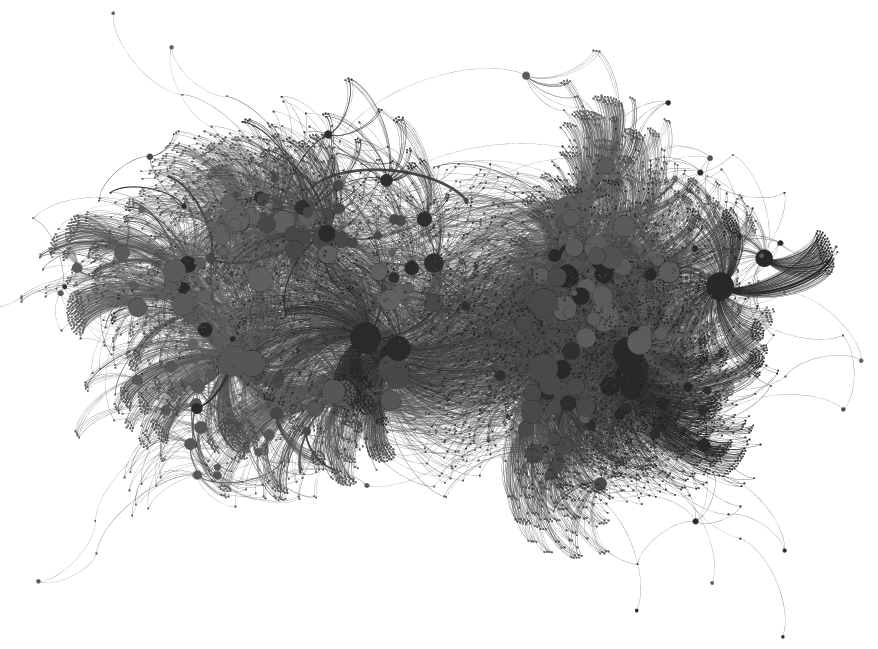
\includegraphics{../tables_and_figures/fig_1_greyscale_white.png}
\caption{Donor Motivation Models}
\end{figure}

\hypertarget{methodology}{%
\section{Methodology}\label{methodology}}

\(H_{1}\) and \(H_{3}\) test the relationships between the social media
dataset and the political donation dataset. A Granger causality
time-series model was used to test the two models of political donor
motivations. Other social media studies have used this methodology
(Freelon, McIlwain, and Clark 2018; Lukito 2020). Similar to political
donations, this methodology has been used to study the relationship
between social media and non-social media events such as offline
protests (Bastos, Mercea, and Charpentier 2015) and stock prices (Park,
Leung, and Ma 2017). Granger causality detects whether movements in one
time series precedes, lags, has a confounding variable, or is not
related to another time series (Granger 1969). An abbreviated version of
how this methodology works is that one takes two time series variables X
and Y. First, a vector autoregression (VAR) model is built to predict
the outcome variable Y with Y being the sole predictor of the model. In
other words, one only uses Y to predict Y. Then, a second model is built
where both variables X and Y are used to build the VAR to predict Y.
Effectively, if the second model, with the inclusion of X, does a better
job of predicting Y than the first model alone, as measured by an
\emph{F}-statistic, X is said to Granger cause Y. The two variables, X
and Y, are also flipped and the same process is done. If the null is
rejected in both instances, then there is likely a confounding variable
Z. This analysis was conducted in R (R Core Team 2013) with the
\texttt{lmtest} package (Zeileis and Hothorn 2002). P-values were
adjusted with the Bonferroni method (Haynes 2013). The optimal lag for
each model was calculated using a Bayesian Information Criteria
(Ahelegbey, Billio, and Casarin 2016) implemented by the \texttt{tsDyn}
package (Stigler 2010).

We compare time series of donations from clusters of political donors
and time series of the number of social media posts by each topic that
were made by campaigns that each donor cluster contributed to. In other
words, a time series of donations from a donor coalition was compared to
the aggregate count of posts about a given topic made by candidates that
the donor cluster contributed to. For example, donations from donor
coalition 6 Granger caused politicians that received donations from the
coalition to publicly support women's issue and pro-choice policies.
Stated another way, donations from coalition 6 predict whether
candidates will publicly support pro-women policies. The theoretical
connection to political donor psychology is that this behavior is
expected under the access-oriented model of political donor motivations.
Coalitions and policy topics that are accepted by either \(H_{1}\) or
\(H_{3}\) are in Table 1. The full results of the Granger causality
tests are visualized in Figure 2.

\begin{longtable}[]{@{}rllrrl@{}}
\caption{H1 and H3 acceptances}\tabularnewline
\toprule
coalition & policy topic & model & BIC & F-statistic &
p-value\tabularnewline
\midrule
\endfirsthead
\toprule
coalition & policy topic & model & BIC & F-statistic &
p-value\tabularnewline
\midrule
\endhead
0 & veterans issues: bipartisan & consumption & 5 & 7.6 &
\textless.001\tabularnewline
1 & veterans issues: bipartisan & access & 7 & 7.1 &
\textless.001\tabularnewline
1 & drug abuse: bipartisan & consumption & 7 & 4.5 &
\textless.001\tabularnewline
3 & race issues: liberal & access & 4 & 6.7 &
\textless.001\tabularnewline
4 & guns: conservative & consumption & 4 & 6.5 &
\textless.001\tabularnewline
6 & abortion and women's issues: conservative & access & 2 & 14.2 &
\textless.001\tabularnewline
7 & drug abuse: bipartisan & consumption & 7 & 5.7 &
\textless.001\tabularnewline
11 & infrastructure: liberal & consumption & 7 & 5.8 &
\textless.001\tabularnewline
\bottomrule
\end{longtable}

\begin{figure}
\centering
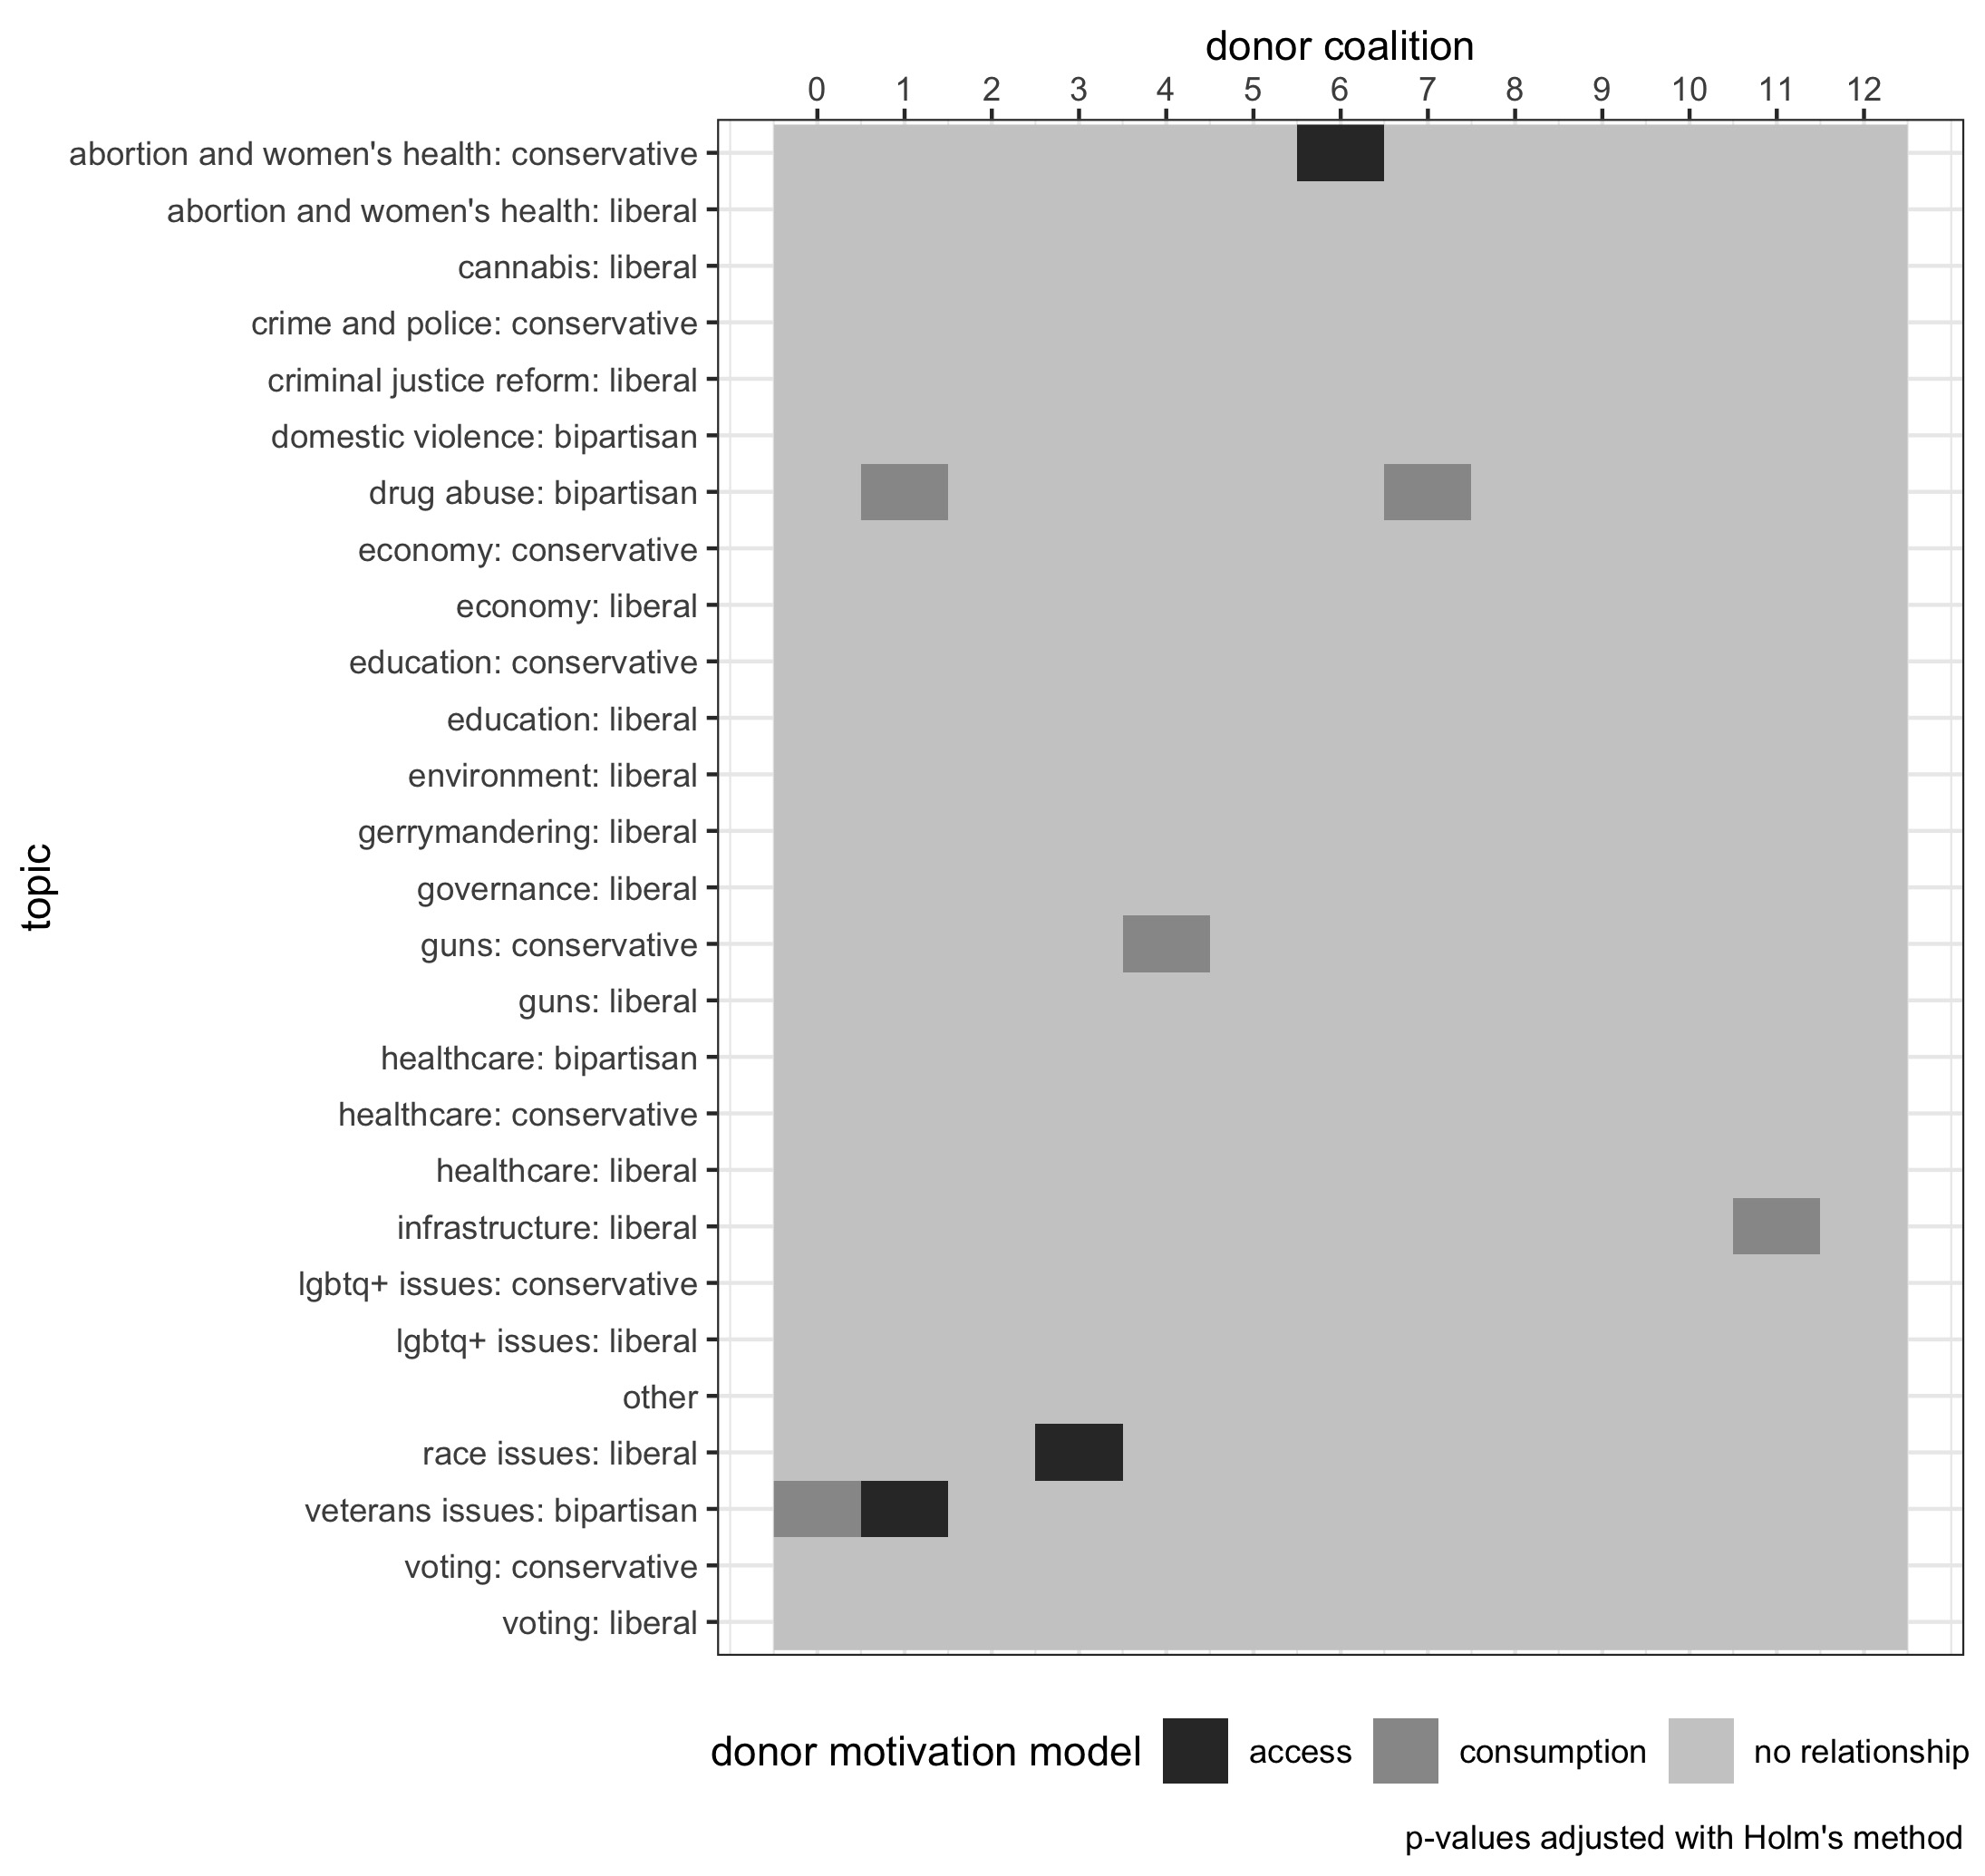
\includegraphics{../tables_and_figures/fig_2.jpg}
\caption{Donor Motivation Models}
\end{figure}

These results were used to test \(H_{1}\) and \(H_{3}\). Donor
coalitions and the topic of social media posts that were accepted by
\(H_{1}\) and \(H_{3}\) are listed in Table 1. Coalitions of donors that
were accepted by only \(H_{1}\) or \(H_{3}\) were used to test \(H_{2}\)
and \(H_{4}\) with a difference-in-means permutation test since the
statistical assumptions were not met for an OLS regression. Results to
\(H_{2}\) and \(H_{4}\) are in Table 2.

To study the polarization of consumption-motivated donors, we extract
the x-coordinate position from the donor network (Figure 1). We then
rescale the coordinate position to be -1 to 1 with -1 representing the
left-most, or most Democratic, node and 1 representing the right-most,
or most Republican, node. To test \(H_{5}\) and \(H_{6}\), a
difference-in-means permutation test on the absolute value of the
rescaled x-coordinate with the coalition category as a variable. A
non-parametric permutation test was used since the statistical
assumptions for an OLS regression were not met. This absolute value
effectively is the level of polarization in the graph, with the nodes
that are on the extremes of the graph being closer to 1 and the
central-most nodes, representing bipartisan donors, being closer to 0.
Results for \(H_{5}\) and \(H_{6}\) are in Table 3.

\hypertarget{results}{%
\section{Results}\label{results}}

We find evidence that supports the recent scholarship into the
motivations of political donors that maintains a nuanced view into the
psychology of political contributors: different donors hold different
motivations. Different donor coalitions exhibited behavior that is
inline with both the access-oriented and consumption model of political
donations with policy issues across the ideological spectrum of liberal,
conservative, and bipartisan. Example social media posts of the various
topics can be found in the appendix.

\hypertarget{access-oriented-coaltiions}{%
\section{Access-oriented Coaltiions}\label{access-oriented-coaltiions}}

For three donor coalitions show behavior consistent with the
access-oriented model where we can predict politicians' public support
of policy issues after they receive contributions from these donor
groups. For these three groups and policy issues \(H_{1}\) is accepted.
These access-oriented coalitions represent 1,572 individual donors or
21.3\% of all donors in the dataset; 6,489 individual donations or
22.4\% of donations; and \$654,577.60 or 16.5\% of dollars contributed.
Each of these three coalitions appear to have unique policy and even
ideological positions that they support.

\hypertarget{race-issues}{%
\subsection{Race Issues}\label{race-issues}}

Donations from donor coalition 3 Granger caused politicians they
contributed to to talk about liberal policies on race. Some social media
posts talk about broader cultural issues as they relate to race
(appendix example 1) and others discuss evidence and propose policies to
address racial issues (appendix example 2). Race was a big part of the
2016 presidential campaign, and racial issues were also a topic in this
dataset. This coalition contains 423 donors or 5.7\% of all donors in
this dataset.

\hypertarget{pro-life}{%
\subsection{Pro-life}\label{pro-life}}

Coalition 6's donations predicts politicians' support for conservative
policies on abortion and women's health, pro-life policies. Some posts
explicitly talk about pro-life organizations and the politicians'
support of those organizations, other posts talk about specific policies
and where the legislative process, and others still are
campaign-oriented appeals that use more coded language that the BERT
model was still able to pickup on (appendix examples 3, 4, and 5,
respectively). Pro-life policies are a perennial topic in Wisconsin
elections. This donor coalition is one of the smaller clusters of donors
with only 252 donors or 3.4\% of donors.

\hypertarget{veterans-issues}{%
\subsection{Veteran's Issues}\label{veterans-issues}}

The final access-oriented group of donors, coalition 1, have donations
that precede politicians posting about bipartisan veteran's issues.
Veteran's issues were particularly salient during the 2016 election in
Wisconsin with Veteran's Affairs hospitals, specifically the Tomah,
Wisconsin VA Hospital and one Wisconsin-run housing complex, Wisconsin
Veteran's Home At King, receiving a lot of public attention for poor
management and other issues. Both Republicans (appendix example 6) and
Democrats (appendix example 7) publicly supported various policies and
initiatives aimed to assist veterans. This coalition contains the second
most donors, 897, or 12.1\% of all donors.

\hypertarget{consumption-oriented-coalitions}{%
\section{Consumption-oriented
Coalitions}\label{consumption-oriented-coalitions}}

In addition to these three access-oriented clusters of donors, five
coalitions of donors exhibit behavior that one would expect under the
consumption model of donor motivations and are accepted by \(H_{3}\). In
other words, public support of various policy issues from campaigns
predicts donations from these coalitions. The five consumption-motivated
clusters of donors contain: 2,702, 36.7\% of donors; 11,080, 38.4\% of
donations; and donated a collective \$1,341,129.70 or 33.8\% of money
contributed. Similar to access-oriented clusters, consumption-oriented
coalitions show significant relationships to policy issues across the
ideological spectrum.

\hypertarget{pro-gun}{%
\subsection{Pro-gun}\label{pro-gun}}

One consumption-oriented group, coalition4, shows a relationship with
conservative gun-related policies where pro-gun public support Granger
causes donations from this group. In other words, donations from this
coalition of donor can be predicted by politicians publicly supporting
conservative gun-related policies. Social media posts that are
categorized as being supportive of conservative policies on gun-related
issues range from talking about their relationship to pro-gun interest
groups (appendix example 8) as well as specific policies (appendix
example 9). This coalition is medium-sized with 605 donors or 8.2\% of
the total donors.

\hypertarget{infrastructure-and-roads}{%
\subsection{Infrastructure and roads}\label{infrastructure-and-roads}}

In addition to a conservative consumption-oriented group, coalition 11
is a group of donors consumptive group of donors whose donations can be
predicted by politicians publicly supporting liberal measure on public
infrastructure and roads. Most of these posts are either general support
of public infrastructure improvements (appendix example 10) or targeted
Republican Governor Scott Walker and Republicans over roads containing a
large number of pot holes (appendix example 11). There are 395 donors in
the coalition or 5.4\% of donors.

\hypertarget{veterans-issues-drug-abuse}{%
\subsection{Veteran's Issues \& Drug
Abuse}\label{veterans-issues-drug-abuse}}

Two different bipartisan policy issues Granger cause donations from two
different coalitions. Coalition 0 (377 donors, 5.1\% of donors) has a
consumption-oriented relationship with politicians' support of veteran's
issues. This topic, veterans issue, had a different coalition of donors
that display an access-oriented relationship with the topic. Both a
consumption-oriented and an access-oriented group displaying a
relationship to the same topic is noteworthy. In addition, the donor
coalition that showed the access-oriented relationship to veterans
issues, coalition 1, also exhibited a consumption-oriented relationship
to another bipartisan issue, drug abuse. While it is just a singular
example, this datum suggests that political donors can have different
motivations with different policies, for example, they can be
access-oriented on veterans issues and consumption-oriented on drug
abuse issues. Another coalition of 428 donors, representing 5.8\% of
donors, also had a significant consumptive relationship with drug abuse.
Most posts about drug abuse focused on the opioid and heroin epidemic
across Wisconsin (appendix example 12). The implications of these
statistical patterns are addressed further in the discussion section.

\hypertarget{donor-sizes}{%
\section{Donor Sizes}\label{donor-sizes}}

Neither the access-oriented donors nor the consumption-oriented donors
contributed statistically significantly different amounts of money than
donors that were donors that were not only access-oriented and not only
consumption-oriented. The outputs of the bootstrap used to test
\(H_{2}\), that access-oriented donors are on-average larger donors, and
\(H_{4}\), that consumption-oriented donors are on-average smaller
donors, are in Table 2. Both \(H_{2}\) and \(H_{4}\) are not accepted.
This finding is discussed in the next section of the paper.

\begin{longtable}[]{@{}llrlr@{}}
\caption{Difference in Average Donor Size}\tabularnewline
\toprule
Hypothesis & Model & T & 95\% CI & p-value\tabularnewline
\midrule
\endfirsthead
\toprule
Hypothesis & Model & T & 95\% CI & p-value\tabularnewline
\midrule
\endhead
H2 & access & -48.62 & -115.4-21.47 & 0.144\tabularnewline
H4 & consumption & 34.60 & -29.21-118.39 & 0.310\tabularnewline
\bottomrule
\end{longtable}

\hypertarget{donor-spatial-positions}{%
\section{Donor Spatial Positions}\label{donor-spatial-positions}}

Consumption-motivated donors are on average in more polarized positions
(further to the left and right of the graph) than
non-consumption-oriented donors, and access-oriented donors are on
average in less polarized positions (closer to the middle of the graph)
than non-access-oriented donors. Table 3 shows the output for \(H_{5}\),
that consumption-oriented donors are more polarized in the network
graph, and \(H_{6}\), that access-oriented donors are less polarized in
the network graph. Both of these hypotheses are accepted. These results
are discussed further in the next section.

\begin{longtable}[]{@{}llrll@{}}
\caption{Difference in Average Donor Position
Polarization}\tabularnewline
\toprule
Hypothesis & Model & T & 95\% CI & p-value\tabularnewline
\midrule
\endfirsthead
\toprule
Hypothesis & Model & T & 95\% CI & p-value\tabularnewline
\midrule
\endhead
H5 & consumption & 0.01 & 0-0.02 & 0.014\tabularnewline
H6 & access & -0.05 & -0.06--0.03 & \textless.001\tabularnewline
\bottomrule
\end{longtable}

\hypertarget{discussion}{%
\section{Discussion}\label{discussion}}

The analyses conducted in this paper show that multiple models of
political donor motivations can exist within different coalitions of
political donors. Historical studies on the motivations of political
donors have explicitly reasoned or implicitly assumed that donors hold
monolithic motivations--all donors are motivated by the same
psychological processes. The results of this paper contrast this
historical principle and instead is in agreement with the recent line of
donor studies which take a more nuanced approach to political donors.

While much of the popular concern over money in politics is around
access-oriented donors manipulating the political system, we find that
there are more consumption-oriented donors than access-oriented donors.
There are more consumption-motivated groups of donors than
access-oriented donors, five groups compared to three, respectively.
These group consumptive groups also represent more people (2,702 versus
1,572), donations (11,080 versus 6,489), and total amount contributed
(\$1,341,129.70 versus \$654,577.60). While any number of
access-oriented donors may remain concerning to some in the public,
these results suggest that more people use political donations as a
vehicle for increased participation, not manipulation, of the political
process.

The folk theory of political donors is that of access-oriented donors
with financial interests donating large sums of money to politicians,
but the results of \(H_{2}\) reject this idea. Donors in access-oriented
coalitions do not contribute statistically significantly more money on
average than other donors. Just because a donor is not contributing a
large sum of money themselves does not mean that they are not seeking to
coax a politician into supporting specific policies. This effect can be
amplified when coalitions of donors operate in conjunction with one
another. For example, members of an interest group could each contribute
a relatively small amount of money, but in aggregate, the unified
donations could potentially gain that interest group access to a
politician. If anything, donors that are labeled in this study as being
in an access-oriented cluster potentially donate less money than other
donors, but this non-statistically significant result with a relatively
large confidence interval is not conclusive. A future study could
replicate this analysis with multiple election cycles or study multiple
states or federal elections to achieve higher statistical power. The
converse is found for consumption-oriented donors.

The folk theory of consumption-motivated donors is of small-dollar
donors whose contributions can be harnessed online. Similar to
access-oriented donors, \(H_{4}\) is rejected and consumption-motivated
donors are not on average smaller donors than other contributors. Again,
these results suggests a disaggregation between the notion that the
amount of money one contributes is indicative of one's motivations. If
someone is able to to contribute a large sum of money and they care
about a certain issue, it stands to reason that they may just support
campaigns who already care about that issue. If contributions to
campaigns are similar to financial investments, the equivalent is
someone investing in a company because they believe the company will do
well in the future, not because every time someone invests in a company
they expect to be able to tangibly alter the direction of the company.
While there are certainly activist investors, they are well outnumbered
by the amount of people who are not activist investors, even among
wealthy individuals. This paper challenges conventional beliefs on the
size of access-oriented versus consumptive donors, but it does concur
with the literature on the levels of polarization among donors.

Consumption-motivated donors are in more polarized spatial positions
within the donor graph than non-consumptive donors, and access-oriented
donors are more centrally located. The acceptances of \(H_{5}\) and
\(H_{6}\) are in agreement with past literature. These results provide
descriptive context and are not meant to imply any level of causality.
Past studies have either suggested or found a connection between donor
motivations and political polarization, and this study also finds these
descriptive relationships. Future studies should examine the causal
mechanisms of these relationships. Do candidates take more polarizing
stances in an effort to court consumptive donors? Has an increased
number of consumptive donors helped more polarized candidates to win
office? Do access-oriented donors seek out campaigns that are more
moderate? Or can access-oriented donors influence the ideological
extremity of candidates?

In addition to the finding that both the access-oriented and consumption
motivational models can exist in different donor coalitions, one of the
thirteen donor clusters, coalition 1, revealed a duality where they were
access-oriented in relation to one policy issue and consumption-oriented
to another. While it is possible that this finding is spurious, there is
additional face validity in this finding because the two issues the
donor coalition had a relationship with were both bipartisan
issues--veterans issues and drug abuse. Not many studies have come to
the conclusion that donors can operate with both motivational models.
While this study finds this behavior to be relatively rare, in only one
donor cluster, it does open up the possibilities to an even more complex
view as to why donors make a political contribution. Further, public
support of one policy issue, veteran's issues, is both Granger caused by
donations from a coalition and Granger causes another coalition to make
a contribution. This result suggests that issues can play different
roles to different groups of political donors. One group of donors can
seek access in order to influence that policy, and another group can
display consumptive behavior and reward politicians who already publicly
support policy issues.

\hypertarget{limitations}{%
\section{Limitations}\label{limitations}}

Like all observational studies, this research cannot claim true
causality. While the main methodology employed is formally called
``Granger causality,'' this causality is in an econometric sense and is
more akin to predictive value. So while the findings of this paper do
have predictive power--for example, donations from certain groups of
individuals successfully receiving candidates to publicly support policy
issues--true causal claims cannot be made. Future studies should use the
findings from this research to conduct lab experiments where causal
claims can be made.

We found discrete examples of donor coalitions demonstrating
access-oriented or consumptive behavior on specific issues. However,
these results do not suggest that these donors only care about those
issues or that other donors don't care about these issues. Instead,
these donors have a unique statistical relationship where when they
contribute money to a political campaign, it either predicts or is
predicted by campaigns public support of policy issues. Future studies
can employ surveys to identify if the statistical relationships found in
an analysis like this paper concur with people's self conceptions. Do
donor coalitions who donate in a consumptive fashion where they
contribute to a campaign after they publicly support an issue actually
report that they prioritize that issue? Possibly, these behaviors are
subconscious reactions. Donors may not be able to exactly identify
\emph{why} they like a candidate or may report some other reason, when
it is actually a reinforcement of a concurrence between their policies
and the information environment that they consume.

Finally, this study was not meant to find nor did it find exhaustive
evidence as to what motivates ever single donor in the dataset. Even
within the information ecology, this study does not consider things like
news stories or personal friend circles. There are other potential
reasons that donors make contributions, such as geographic proximity
where people donate to their local candidates or allocating money to
competitive races.

\hypertarget{conclusion}{%
\section{Conclusion}\label{conclusion}}

Campaign finance scholars are divided on the motivations of political
donors. Do political donors seek to buy access, to participate more in
politics, or some combination of both? This study finds that different
coalitions of donors, and in one instance, a singular coalition, exhibit
behavior that is consistent with different motivational models. Overall,
there are more consumptive donors compared to access-oriented donors. In
addition, there is no statistical difference in the average contributor
size of access-oriented and consumption-oriented donors compared to
other donors. However, access-oriented donors are found to be more
spatially central within donor networks, and consumptive donors are more
polarized.

\hypertarget{appendix}{%
\section{Appendix}\label{appendix}}

\begin{longtable}[t]{>{\raggedright\arraybackslash}p{.65in}|>{\raggedright\arraybackslash}p{.6in}|>{\raggedright\arraybackslash}p{.7in}|>{\raggedright\arraybackslash}p{.6in}|>{\raggedright\arraybackslash}p{3in}}
\caption{\label{tab:unnamed-chunk-6}Social Media Examples}\\
\hline
example \# & topic & campaign & social media site & post\\
\hline
\endfirsthead
\caption[]{Social Media Examples \textit{(continued)}}\\
\hline
example \# & topic & campaign & social media site & post\\
\hline
\endhead
1 & race issues: liberal & Bowen 4 Action & Twitter & @ JoyAnnReid: \#OscarsSoWhite black people can't even get nominated for the movies about black people...\\
\hline
2 & race issues: liberal & Citizens of the 81st for Dave Considine & Twitter & 1 in every 9 African-Americans are disenfranchised because of felony convictions in Wisconsin\\
\hline
3 & abortion and women's issues: conservative & Ken Skowronski for Assembly & Facebook & Last night I had a great time at the Wisconsin Right to Life Dinner with my fellow colleagues. I am proud to have supported the bold Pro-Life reforms we have put in place and I will continue to defend the rights of those who cannot defend themselves.\\
\hline
4 & abortion and women's issues: conservative & Friends \& Neighbors of Robin Vos & Twitter & An Assembly committee will vote on a bill to ban the sale of aborted children's body parts on Wednesday.\\
\hline
5 & abortion and women's issues: conservative & Friends of Chuck Wichgers & Facebook & 'I'm glad to know Chuck, who is a solid conservative. He's shown that he understands the principles that secure our freedom and that he will work for them in office. But more than that, I've seen that he is passionate about the God-given dignity of every human life. He knows that every person's right to live and to live freely comes from a much higher source than government.'PATRICK MCILHERAN, FORMER EDITORIAL WRITER, MILWAUKEE JOURNAL SENTINEL\\
\hline
6 & veterans issues: bipartisan & Sanfelippo for Assembly & Twitter & Welcome Home Veterans Initiative seeks to solve veteran homelessness in state:\\
\hline
7 & veterans issues: bipartisan & Citizens for Peter Barca & Twitter & Regionalizing Wisconsin's county veterans service offices remains a concern in vet community\\
\hline
8 & guns: conservative & Scott Fitzgerald for Senate & Twitter & Thanks to the Wisconsin Game Preserve Association for the honor of their 2015 Legislator of the Year award!\\
\hline
9 & guns: conservative & Kremer for Wisconsin & Facebook & This is a fair interview with Frederica Freyberg discussing the 'Campus Carry Act' in Wisconsin.  This aired on public television yesterday morning.\\
\hline
10 & infrastructure: liberal & Friends of Jonathan Brostoff & Facebook & Dr. Mark Stout has written a compelling alternative to the \$1.1 billion highway proposal. This option that would save money and provide a brighter, more progressive, more responsible future for our state. If you haven't yet, please take a look and share widely.\\
\hline
11 & infrastructure: liberal & Wachs for Assembly & Twitter & WI roads rank 3rd worst in US. Yet Scott Walker isnt ready to put politics aside to solve our infrastructure woes.\\
\hline
12 & drug abuse: bipartisan & Michael Schraa for Assembly & Facebook & A great story about the HOPE Agenda and my colleague on Joint Finance, WI State Rep John Nygren's efforts to fight against heroin and opiate addiction.\\
\hline
\end{longtable}

\begin{tabular}{l|l|l}
\hline
Method & koRpus & stringi\\
\hline
Word count & 7681 & 7610\\
\hline
Character count & 51899 & 51888\\
\hline
Sentence count & 367 & Not available\\
\hline
Reading time & 38.4 minutes & 38 minutes\\
\hline
\end{tabular}

\hypertarget{references}{%
\section*{References}\label{references}}
\addcontentsline{toc}{section}{References}

\hypertarget{refs}{}
\leavevmode\hypertarget{ref-bic}{}%
Ahelegbey, Daniel Felix, Monica Billio, and Roberto Casarin. 2016.
``Bayesian Graphical Models for Structural Vector Autoregressive
Processes.'' \emph{Journal of Applied Econometrics} 31 (2): 357--86.
\url{https://doi.org/https://doi.org/10.1002/jae.2443}.

\leavevmode\hypertarget{ref-akey2015}{}%
Akey, Pat. 2015. ``Valuing Changes in Political Networks: Evidence from
Campaign Contributions to Close Congressional Elections.'' \emph{The
Review of Financial Studies} 28 (11): 3188--3223.
\url{https://doi.org/10.1093/rfs/hhv035}.

\leavevmode\hypertarget{ref-albert2020}{}%
Albert, Zachary, and Raymond La Raja. 2020. ``Small Dollar Donors and
the Evolving Democratic Party.'' \emph{APSA Preprints}.

\leavevmode\hypertarget{ref-anduiza2010}{}%
Anduiza, Eva, Aina Gallego, and Marta Cantijoch. 2010. ``Online
Political Participation in Spain: The Impact of Traditional and Internet
Resources.'' \emph{Journal of Information Technology \& Politics} 7 (4):
356--68. \url{https://doi.org/10.1080/19331681003791891}.

\leavevmode\hypertarget{ref-ansolabehere2003}{}%
Ansolabehere, Stephen, John M. de Figueiredo, and James M. Snyder. 2003.
``Why Is There so Little Money in U.s. Politics.'' \emph{Journal of
Economic Perspectives} 17 (1): 105--30.

\leavevmode\hypertarget{ref-arbour2020}{}%
Arbour, Brian. 2020. ``Tiny Donations, Big Impact: How Small-Dollar
Donors Are Eroding the Power of Party Insiders.'' \emph{Society} 57:
496--506.

\leavevmode\hypertarget{ref-austensmith1995}{}%
Austen-Smith, David. 1995. ``Campaign Contributions and Access.''
\emph{The American Political Science Review} 89 (3): 566--81.
\url{http://www.jstor.org/stable/2082974}.

\leavevmode\hypertarget{ref-baker2020a}{}%
Baker, Anne. 2020a. ``Policies, Profits, Networks, or Duty?: Donors'
Motivations for Contributing to Parties and Interest Groups.'' \emph{The
Social Science Journal} 0 (0): 1--16.
\url{https://doi.org/10.1080/03623319.2020.1727224}.

\leavevmode\hypertarget{ref-baker2020b}{}%
---------. 2020b. ``The Partisan and Policy Motivations of Political
Donors Seeking Surrogate Representation in House Elections.''
\emph{Political Behavior} 42 (4): 1035--54.
\url{https://doi.org/10.1007/s11109-019-09531-2}.

\leavevmode\hypertarget{ref-barber2016a}{}%
Barber, Michael. 2016. ``Donation Motivations: Testing Theories of
Access and Ideology.'' \emph{Political Research Quarterly} 69 (1):
148--59.

\leavevmode\hypertarget{ref-barber2019}{}%
Barber, Michael, Brandice Canes-Wrone, and Sharece Thrower. 2019.
``Campaign Contributions and Donors' Policy Agreement with Presidential
Candidates.'' \emph{Presidential Studies Quarterly} 49 (4): 770--97.
\url{https://doi.org/https://doi.org/10.1111/psq.12609}.

\leavevmode\hypertarget{ref-barber2017}{}%
Barber, Michael J., Brandice Canes-Wrone, and Sharece Thrower. 2017.
``Ideologically Sophisticated Donors: Which Candidates Do Individual
Contributors Finance?'' \emph{American Journal of Political Science} 61
(2): 271--88. \url{https://doi.org/https://doi.org/10.1111/ajps.12275}.

\leavevmode\hypertarget{ref-rfacebook}{}%
Barbera, Pablo, Andrew Geisler, and Wouter van Atteveldt. 2017.
\emph{Rfacebook}.
\url{https://cran.r-project.org/web/packages/Rfacebook/Rfacebook.pdf}.

\leavevmode\hypertarget{ref-gephi}{}%
Bastian, Mathieu, Sebastien Heymann, and Mathieu Jacomy. 2009. ``Gephi:
An Open Source Software for Exploring and Manipulating Networks.''
\url{http://www.aaai.org/ocs/index.php/ICWSM/09/paper/view/154}.

\leavevmode\hypertarget{ref-bastos2015}{}%
Bastos, Marco T., Dan Mercea, and Arthur Charpentier. 2015. ``Tents,
Tweets, and Events: The Interplay Between Ongoing Protests and Social
Media.'' \emph{Journal of Communication} 65 (2): 320--50.
\url{https://doi.org/10.1111/jcom.12145}.

\leavevmode\hypertarget{ref-benoit2019}{}%
Benoit, Kenneth, Kevin Munger, and Arthur Spirling. 2019. ``Measuring
and Explaining Political Sophistication Through Textual Complexity.''
\emph{American Journal of Political Science} 63 (2): 491--508.
\url{https://doi.org/https://doi.org/10.1111/ajps.12423}.

\leavevmode\hypertarget{ref-bonica2014}{}%
Bonica, Adam. 2014. ``Mapping the Ideological Marketplace.''
\emph{American Journal of Political Science} 58 (2): 367--86.
\url{http://www.jstor.org/stable/24363491}.

\leavevmode\hypertarget{ref-bonica2016}{}%
---------. 2016. ``Avenues of Influence: On the Political Expenditures
of Corporations and Their Directors and Executives.'' \emph{Business and
Politics} 18 (4): 367--94. \url{https://doi.org/10.1515/bap-2016-0004}.

\leavevmode\hypertarget{ref-bonica2019}{}%
---------. 2019. ``Are Donation-Based Measures of Ideology Valid
Predictors of Individual-Level Policy Preferences?'' \emph{The Journal
of Politics} 81 (1): 327--33. \url{https://doi.org/10.1086/700722}.

\leavevmode\hypertarget{ref-butler2011}{}%
Butler, Daniel M., and David W. Nickerson. 2011. ``Can Learning
Constituency Opinion Affect How Legislators Vote? Results from a Field
Experiment.'' \emph{Quarterly Journal of Political Science} 6: 55--83.

\leavevmode\hypertarget{ref-callahan2019}{}%
Callahan, Scott. 2019. ``Do Campaign Contributions from Farmers
Influence Agricultural Policy? Evidence from a 2008 Farm Bill Amendment
Vote to Curtail Cotton Subsidies.'' \emph{Journal of Agricultural and
Applied Economics} 51 (3): 417--33.
\url{https://doi.org/10.1017/aae.2019.9}.

\leavevmode\hypertarget{ref-caneswrone2019}{}%
Canes-Wrone, Brandice, and Nathan Gibson. 2019. ``Does Money Buy
Congressional Love? Individual Donors and Legislative Voting.''
\emph{Congress \& the Presidency} 46 (1): 1--27.
\url{https://doi.org/10.1080/07343469.2018.1518965}.

\leavevmode\hypertarget{ref-chester2017}{}%
Chester, Jeff, and Kathryn C. Montgomery. 2017. ``The Role of Digital
Marketing in Political Campaigns.'' \emph{Internet Policy Review} 6 (4):
1--20. \url{https://doi.org/10.14763/2017.4.773}.

\leavevmode\hypertarget{ref-choma2020}{}%
Choma, Russ, and Kara Voght. 2020. ``Small-Dollar Donors Powered the
2020 Race. Then the Pandemic Happened.'' \emph{Mother Jones}, April.

\leavevmode\hypertarget{ref-cogburn2011}{}%
Cogburn, Derrick L., and Fatima K. Espinoza-Vasquez. 2011. ``From
Networked Nominee to Networked Nation: Examining the Impact of Web 2.0
and Social Media on Political Participation and Civic Engagement in the
2008 Obama Campaign.'' \emph{Journal of Political Marketing} 10 (1-2):
189--213. \url{https://doi.org/10.1080/15377857.2011.540224}.

\leavevmode\hypertarget{ref-constant2006}{}%
Constant, Louay M. 2006. ``When Money Matters: Campaign Contributions,
Roll Call Votes, and School Choice in Florida.'' \emph{State Politics \&
Policy Quarterly} 6 (2): 195--219.
\url{https://doi.org/10.1177/153244000600600204}.

\leavevmode\hypertarget{ref-cooper2010}{}%
Cooper, Michael J., Huseyin Gulen, and Alexei V. Ovtchinnikov. 2010.
``Corporate Political Contributions and Stock Returns.'' \emph{The
Journal of Finance} 65 (2): 687--724.
\url{https://doi.org/https://doi.org/10.1111/j.1540-6261.2009.01548.x}.

\leavevmode\hypertarget{ref-cranshaw2010}{}%
Cranshaw, Justin, Eran Toch, J. Hong, A. Kittur, and N. Sadeh. 2010.
``Bridging the Gap Between Physical Location and Online Social
Networks.'' \emph{Proceedings of the 12th ACM International Conference
on Ubiquitous Computing}.

\leavevmode\hypertarget{ref-culberson2019}{}%
Culberson, Tyler, Michael P. McDonald, and Suzanne M. Robbins. 2019.
``Small Donors in Congressional Elections.'' \emph{American Politics
Research} 47 (5): 970--99.
\url{https://doi.org/10.1177/1532673X18763918}.

\leavevmode\hypertarget{ref-bert}{}%
Devlin, Jacob, Ming-Wei Chang, Kenton Lee, and Kristina Toutanova. 2019.
``BERT: Pre-Training of Deep Bidirectional Transformers for Language
Understanding.'' \url{http://arxiv.org/abs/1810.04805}.

\leavevmode\hypertarget{ref-marx2000}{}%
DSW, Jerry D. Marx. 2000. ``Online Fundraising in the Human Services.''
\emph{Journal of Technology in Human Services} 17 (2-3): 137--52.
\url{https://doi.org/10.1300/J017v17n02/_03}.

\leavevmode\hypertarget{ref-edwards2016}{}%
Edwards, Geoff, and Rui de Figueiredo. 2016. ``The Market for
Legislative Influence over Regulatory Policy'' 34 (May).
\url{https://doi.org/10.1108/S0742-332220160000034007}.

\leavevmode\hypertarget{ref-ellison2006}{}%
Ellison, Nicole, and Charles Steinfield. 2006. ``Spatially Bounded
Online Social Networks and Social Capital: The Role of Facebook.''
\emph{Annual Conference of the International Communication Association},
January.

\leavevmode\hypertarget{ref-engel1998}{}%
Engel, Steven T., and David J. Jackson. 1998. ``Wielding the Stick
Instead of the Carrot: Labor Pac Punishment of Pro-Nafta Democrats.''
\emph{Political Research Quarterly} 51 (3): 813--28.
\url{https://doi.org/10.1177/106591299805100312}.

\leavevmode\hypertarget{ref-ensley2009}{}%
Ensley, Michael J. 2009. ``Individual Campaign Contributions and
Candidate Ideology.'' \emph{Public Choice} 138 (1/2): 221--38.
\url{http://www.jstor.org/stable/40270840}.

\leavevmode\hypertarget{ref-fellowes2004}{}%
Fellowes, Matthew C., and Patrick J. Wolf. 2004. ``Funding Mechanisms
and Policy Instruments: How Business Campaign Contributions Influence
Congressional Votes.'' \emph{Political Research Quarterly} 57 (2):
315--24.

\leavevmode\hypertarget{ref-ferris2019}{}%
Ferris, Stephen P., Reza Houston, and David Javakhadze. 2019. ``It Is a
Sweetheart of a Deal: Political Connections and Corporate-Federal
Contracting.'' \emph{Financial Review} 54 (1): 57--84.
\url{https://doi.org/https://doi.org/10.1111/fire.12181}.

\leavevmode\hypertarget{ref-finger2019}{}%
Finger, Leslie K. 2019. ``Interest Group Influence and the Two Faces of
Power.'' \emph{American Politics Research} 47 (4): 852--86.
\url{https://doi.org/10.1177/1532673X18786723}.

\leavevmode\hypertarget{ref-fouirnaies2018}{}%
Fouirnaies, Alexander. 2018. ``When Are Agenda Setters Valuable?''
\emph{American Journal of Political Science} 62 (1): 176--91.
\url{https://doi.org/https://doi.org/10.1111/ajps.12316}.

\leavevmode\hypertarget{ref-fouirnaies2015}{}%
Fouirnaies, Alexander, and Andrew Hall. 2015. ``The Exposure Theory of
Access: Why Some Firms Seek More Access to Incumbents Than Others.''
\emph{SSRN Electronic Journal}, January.
\url{https://doi.org/10.2139/ssrn.2652361}.

\leavevmode\hypertarget{ref-francia2003}{}%
Francia, Peter L., John C. Green, Paul S. Herrnson, Lynda W. Powell, and
and Clyde Wilcox. 2003. \emph{The Financiers of Congressional
Elections}. New York, NY: Columbia University Press.

\leavevmode\hypertarget{ref-freelon2018}{}%
Freelon, D, C McIlwain, and M Clark. 2018. ``Quantifying the Power and
Consequences of Social Media Protest.'' \emph{New Media \& Society} 20
(3): 990--1011. \url{https://doi.org/10.1177/1461444816676646}.

\leavevmode\hypertarget{ref-fremeth2013}{}%
Fremeth, Adam, Brian Kelleher Richter, and Brandon Schaufele. 2013.
``Campaign Contributions over Ceos' Careers.'' \emph{American Economic
Journal: Applied Economics} 5 (3): 170--88.
\url{https://doi.org/10.1257/app.5.3.170}.

\leavevmode\hypertarget{ref-fu2020}{}%
Fu, Shu, and William G. Howell. 2020. ``The Behavioral Consequences of
Public Appeals: Evidence on Campaign Fundraising from the 2018
Congressional Elections.'' \emph{Presidential Studies Quarterly} 50 (2):
325--47. \url{https://doi.org/https://doi.org/10.1111/psq.12645}.

\leavevmode\hypertarget{ref-fulmer2017}{}%
Fulmer, Sarah, A. Knill, and X. Yu. 2017. ``Negation of Sanctions: The
Personal Effect of Political Contributions.'' \emph{Business History
eJournal}.

\leavevmode\hypertarget{ref-degennaro2006}{}%
Gennaro, Corinna di, and William Dutton. 2006. ``The Internet and the
Public: Online and Offline Political Participation in the United
Kingdom.'' \emph{Parliamentary Affairs} 59 (2): 299--313.
\url{https://doi.org/10.1093/pa/gsl004}.

\leavevmode\hypertarget{ref-zuniga2012}{}%
Gil de Zúñiga, Homero, Nakwon Jung, and Sebastián Valenzuela. 2012.
``Social Media Use for News and Individuals' Social Capital, Civic
Engagement and Political Participation.'' \emph{Journal of
Computer-Mediated Communication} 17 (3): 319--36.
\url{https://doi.org/10.1111/j.1083-6101.2012.01574.x}.

\leavevmode\hypertarget{ref-goet2019}{}%
Goet, Niels D. 2019. ``Measuring Polarization with Text Analysis:
Evidence from the Uk House of Commons, 1811--2015.'' \emph{Political
Analysis} 27 (4): 518--39. \url{https://doi.org/10.1017/pan.2019.2}.

\leavevmode\hypertarget{ref-goldberg2020}{}%
Goldberg, Matthew H., Jennifer R. Marlon, Xinran Wang, Sander van der
Linden, and Anthony Leiserowitz. 2020. ``Oil and Gas Companies Invest in
Legislators That Vote Against the Environment.'' \emph{Proceedings of
the National Academy of Sciences} 117 (10): 5111--2.
\url{https://doi.org/10.1073/pnas.1922175117}.

\leavevmode\hypertarget{ref-goldmacher2020}{}%
Goldmacher, Shane. 2020. ``The 2020 Campaign Is the Most Expensive Ever
(by a Lot).'' \emph{The New York Times Magazine}, October.

\leavevmode\hypertarget{ref-gordon2007}{}%
Gordon, Sanford C., Catherine Hafer, and Dimitri Landa. 2007.
``Consumption or Investment? On Motivations for Political Giving.''
\emph{The Journal of Politics} 69 (4): 1057--72.

\leavevmode\hypertarget{ref-gounopoulos2021}{}%
Gounopoulos, Dimitrios, Khelifa Mazouz, and Geoffrey Wood. 2021. ``The
Consequences of Political Donations for Ipo Premium and Performance.''
\emph{Journal of Corporate Finance} 67: 101888.
\url{https://doi.org/https://doi.org/10.1016/j.jcorpfin.2021.101888}.

\leavevmode\hypertarget{ref-granger}{}%
Granger, C. W. J. 1969. ``Investigating Causal Relations by Econometric
Models and Cross-Spectral Methods.'' \emph{Econometrica} 37 (3):
424--38. \url{http://www.jstor.org/stable/1912791}.

\leavevmode\hypertarget{ref-grenzke1989}{}%
Grenzke, Janet M. 1989. ``PACs and the Congressional Supermarket: The
Currency Is Complex.'' \emph{American Journal of Political Science} 33
(1): 1--24. \url{http://www.jstor.org/stable/2111251}.

\leavevmode\hypertarget{ref-hadani2017}{}%
Hadani, Michael, Jean-Philippe Bonardi, and Nicolas M Dahan. 2017.
``Corporate Political Activity, Public Policy Uncertainty, and Firm
Outcomes: A Meta-Analysis.'' \emph{Strategic Organization} 15 (3):
338--66. \url{https://doi.org/10.1177/1476127016651001}.

\leavevmode\hypertarget{ref-hall1990}{}%
Hall, Richard L., and Frank W. Wayman. 1990. ``Buying Time: Moneyed
Interests and the Mobilization of Bias in Congressional Committees.''
\emph{American Political Science Review} 84 (3): 797--820.
\url{https://doi.org/10.2307/1962767}.

\leavevmode\hypertarget{ref-openrefine}{}%
Ham, Kelli. 2013. ``OpenRefine (Version 2.5). Http://Openrefine.org.
Free, Open-Source Tool for Cleaning and Transforming Data.''
\emph{Journal of the Medical Library} 101 (3): 233--34.

\leavevmode\hypertarget{ref-hanna2013}{}%
Hanna, Alex, Chris Wells, Peter Maurer, Lew Friedland, Dhavan Shah, and
Jörg Matthes. 2013. ``Partisan Alignments and Political Polarization
Online: A Computational Approach to Understanding the French and Us
Presidential Elections.'' In \emph{Proceedings of the 2nd Workshop on
Politics, Elections and Data}, 15--22. PLEAD '13. New York, NY, USA:
Association for Computing Machinery.
\url{https://doi.org/10.1145/2508436.2508438}.

\leavevmode\hypertarget{ref-harden2016}{}%
Harden, Jeffrey J., and Justin H. Kirkland. 2016. ``Do Campaign Donors
Influence Polarization? Evidence from Public Financing in the American
States.'' \emph{Legislative Studies Quarterly} 41 (1): 119--52.
\url{https://doi.org/https://doi.org/10.1111/lsq.12108}.

\leavevmode\hypertarget{ref-hardina2005}{}%
Hardina, Donna. 2005. ``Using the Web to Teach Power Analysis.''
\emph{The Social Policy Journal} 4 (2): 51--68.
\url{https://doi.org/10.1300/J185v04n02/_05}.

\leavevmode\hypertarget{ref-harlow2020}{}%
Harlow, Summer, Danielle K. Kilgo, Ramón Salaverría, and Víctor
García-Perdomo. 2020. ``Is the Whole World Watching? Building a Typology
of Protest Coverage on Social Media from Around the World.''
\emph{Journalism Studies} 21 (11): 1590--1608.
\url{https://doi.org/10.1080/1461670X.2020.1776144}.

\leavevmode\hypertarget{ref-hayes2017}{}%
Hayes, Thomas J. 2017. ``Bankruptcy Reform and Congressional Action: The
Role of Organized Interests in Shaping Policy.'' \emph{Social Science
Research} 64: 67--78.
\url{https://doi.org/https://doi.org/10.1016/j.ssresearch.2016.09.026}.

\leavevmode\hypertarget{ref-bonferroni}{}%
Haynes, Winston. 2013. ``Bonferroni Correction.'' In \emph{Encyclopedia
of Systems Biology}, edited by Werner Dubitzky, Olaf Wolkenhauer,
Kwang-Hyun Cho, and Hiroki Yokota, 154--54. New York, NY: Springer New
York. \url{https://doi.org/10.1007/978-1-4419-9863-7_1213}.

\leavevmode\hypertarget{ref-hazard2003}{}%
Hazard, Brenda L. 2003. ``Online Fundraising at Arl Libraries.''
\emph{The Journal of Academic Librarianship} 29 (1): 8--15.
\url{https://doi.org/https://doi.org/10.1016/S0099-1333(02)00399-3}.

\leavevmode\hypertarget{ref-heberlig2020}{}%
Heberlig, Eric, and Bruce Larson. 2020. ``Gender and Small
Contributions: Fundraising by the Democratic Freshman Class of 2018 in
the 2020 Election.'' \emph{Society} 57: 534--39.
\url{https://doi.org/https://doi.org/10.1007/s12115-020-00528-w}.

\leavevmode\hypertarget{ref-heerwig2016}{}%
Heerwig, Jennifer A. 2016. ``Donations and Dependence: Individual
Contributor Strategies in House Elections.'' \emph{Social Science
Research} 60: 181--98.
\url{https://doi.org/https://doi.org/10.1016/j.ssresearch.2016.06.001}.

\leavevmode\hypertarget{ref-herndon1982}{}%
Herndon, James F. 1982. ``Access, Record, and Competition as Influences
on Interest Group Contributions to Congressional Campaigns.'' \emph{The
Journal of Politics} 44 (4): 996--1019.

\leavevmode\hypertarget{ref-hill2017}{}%
Hill, Seth J., and Gregory A. Huber. 2017. ``Representativeness and
Motivations of the Contemporary Donorate: Results from Merged Survey and
Administrative Records.'' \emph{Political Behavior} 39 (1): 3--29.
\url{https://doi.org/10.1007/s11109-016-9343-y}.

\leavevmode\hypertarget{ref-hogan2020}{}%
Hogan, Robert E. 2020. ``Legislative Voting and Environmental
Policymaking in the American States.'' \emph{Environmental Politics} 0
(0): 1--20. \url{https://doi.org/10.1080/09644016.2020.1788897}.

\leavevmode\hypertarget{ref-yifanhu}{}%
Hu, Yifan. 2005. ``Efficient, High-Quality Force-Directed Graph
Drawing.'' \emph{Mathematica Journal} 10 (1): 37--71.

\leavevmode\hypertarget{ref-jansa2019}{}%
Jansa, Joshua M. 2019. ``You Catch More Flies with Honey: An Analysis of
Pac Punishment and Congressional Vote Switching.'' \emph{Interest Groups
\& Advocacy} 8 (2).

\leavevmode\hypertarget{ref-jansa2018}{}%
Jansa, Joshua M., and Michele M. Hoyman. 2018. ``Do Unions Punish
Democrats? Free-Trade Votes and Labor Pac Contributions, 1999--2012.''
\emph{Political Research Quarterly} 71 (2): 424--39.
\url{https://doi.org/10.1177/1065912917738575}.

\leavevmode\hypertarget{ref-jiang2020}{}%
Jiang, Shan, Miriam Metzger, Andrew Flanagin, and Christo Wilson. 2020.
``Modeling and Measuring Expressed (Dis)belief in (Mis)information.''
\emph{Proceedings of the International AAAI Conference on Web and Social
Media} 14 (1): 315--26.
\url{https://ojs.aaai.org/index.php/ICWSM/article/view/7302}.

\leavevmode\hypertarget{ref-jost2018}{}%
Jost, John, Pablo Barberá, Richard Bonneau, Melanie Langer, Megan
Metzger, Jonathan Nagler, Joanna Sterling, and Joshua Tucker. 2018.
``How Social Media Facilitates Political Protest: Information,
Motivation, and Social Networks: Social Media and Political Protest.''
\emph{Political Psychology} 39 (February): 85--118.
\url{https://doi.org/10.1111/pops.12478}.

\leavevmode\hypertarget{ref-kalla2016}{}%
Kalla, Joshua L., and David E. Broockman. 2016. ``Campaign Contributions
Facilitate Access to Congressional Officials: A Randomized Field
Experiment.'' \emph{American Journal of Political Science} 60 (3):
545--58. \url{https://doi.org/https://doi.org/10.1111/ajps.12180}.

\leavevmode\hypertarget{ref-karpf2010}{}%
Karpf, David. 2010. ``Online Political Mobilization from the Advocacy
Group's Perspective: Looking Beyond Clicktivism.'' \emph{Policy \&
Internet} 2 (4): 7--41.
\url{https://doi.org/https://doi.org/10.2202/1944-2866.1098}.

\leavevmode\hypertarget{ref-rtweet}{}%
Kearney, Michael W. 2019. ``Rtweet: Collecting and Analyzing Twitter
Data.'' \emph{Journal of Open Source Software} 4 (42): 1829.
\url{https://doi.org/10.21105/joss.01829}.

\leavevmode\hypertarget{ref-keena2019}{}%
Keena, Alex, and Misty Knight-Finley. 2019. ``Are Small Donors
Polarizing? A Longitudinal Study of the Senate.'' \emph{Election Law
Journal: Rules, Politics, and Policy} 18 (2): 132--44.
\url{https://doi.org/10.1089/elj.2018.0498}.

\leavevmode\hypertarget{ref-kettler2019}{}%
Kettler, Jaclyn J., and Jeffrey Lyons. 2019. ``The Fickle Financiers of
Elections? The Impact of Moving on Individual Contributions.''
\emph{Journal of Elections, Public Opinion and Parties} 0 (0): 1--19.
\url{https://doi.org/10.1080/17457289.2019.1652620}.

\leavevmode\hypertarget{ref-kreiss2018}{}%
Kreiss, Daniel, and Shannon C. McGregor. 2018. ``Technology Firms Shape
Political Communication: The Work of Microsoft, Facebook, Twitter, and
Google with Campaigns During the 2016 U.s. Presidential Cycle.''
\emph{Political Communication} 35 (2): 155--77.
\url{https://doi.org/10.1080/10584609.2017.1364814}.

\leavevmode\hypertarget{ref-kushin2009}{}%
Kushin, Matthew J., and Kelin Kitchener. 2009. ``Getting Political on
Social Network Sites: Exploring Online Political Discourse on
Facebook.'' \emph{First Monday} 14 (11).
\url{https://doi.org/10.5210/fm.v14i11.2645}.

\leavevmode\hypertarget{ref-langbein1986}{}%
Langbein, Laura I. 1986. ``Money and Access: Some Empirical Evidence.''
\emph{The Journal of Politics} 40 (4): 1052--62.

\leavevmode\hypertarget{ref-lauderdale2016}{}%
Lauderdale, Benjamin E., and Alexander Herzog. 2016. ``Measuring
Political Positions from Legislative Speech.'' \emph{Political Analysis}
24 (3): 374--94. \url{https://doi.org/10.1093/pan/mpw017}.

\leavevmode\hypertarget{ref-lawrence2010}{}%
Lawrence, Eric, John Sides, and Henry Farrell. 2010. ``Self-Segregation
or Deliberation? Blog Readership, Participation, and Polarization in
American Politics.'' \emph{Perspectives on Politics} 8 (1): 141--57.
\url{http://www.jstor.org/stable/25698520}.

\leavevmode\hypertarget{ref-lee2014}{}%
Lee, Jae Kook, Jihyang Choi, Cheonsoo Kim, and Yonghwan Kim. 2014.
``Social Media, Network Heterogeneity, and Opinion Polarization.''
\emph{Journal of Communication} 64 (4): 702--22.
\url{https://doi.org/10.1111/jcom.12077}.

\leavevmode\hypertarget{ref-levenshus2010}{}%
Levenshus, Abbey. 2010. ``Online Relationship Management in a
Presidential Campaign: A Case Study of the Obama Campaign's Management
of Its Internet-Integrated Grassroots Effort.'' \emph{Journal of Public
Relations Research} 22 (3): 313--35.
\url{https://doi.org/10.1080/10627261003614419}.

\leavevmode\hypertarget{ref-liben2005}{}%
Liben-Nowell, David, Jasmine Novak, Ravi Kumar, Prabhakar Raghavan, and
Andrew Tomkins. 2005. ``Geographic Routing in Social Networks.''
\emph{Proceedings of the National Academy of Sciences} 102 (33):
11623--8. \url{https://doi.org/10.1073/pnas.0503018102}.

\leavevmode\hypertarget{ref-lukito2020}{}%
Lukito, Josephine. 2020. ``Coordinating a Multi-Platform Disinformation
Campaign: Internet Research Agency Activity on Three U.s. Social Media
Platforms, 2015 to 2017.'' \emph{Political Communication} 37 (2):
238--55. \url{https://doi.org/10.1080/10584609.2019.1661889}.

\leavevmode\hypertarget{ref-mckay2010}{}%
McKay, Amy. 2010. ``The Effects of Interest Groups' Ideology on Their
Pac and Lobbying Expenditures.'' \emph{Business and Politics} 12 (2):
1--21. \url{https://doi.org/10.2202/1469-3569.1306}.

\leavevmode\hypertarget{ref-mckay2018}{}%
---------. 2018. ``What Do Campaign Contributions Buy? Lobbyists'
Strategic Giving.'' \emph{Interest Groups \& Advocacy} 7 (1).

\leavevmode\hypertarget{ref-milbrath1958}{}%
Milbrath, Lester W. 1958. ``The Political Party Activity of Washington
Lobbyists.'' \emph{The Journal of Politics} 20 (2): 339--52.

\leavevmode\hypertarget{ref-miller2009}{}%
Miller, Bryan. 2009. ``Community Fundraising 2.0---the Future of
Fundraising in a Networked Society?'' \emph{International Journal of
Nonprofit and Voluntary Sector Marketing} 14 (4): 365--70.
\url{https://doi.org/https://doi.org/10.1002/nvsm.373}.

\leavevmode\hypertarget{ref-mozafari2020}{}%
Mozafari, Marzieh, Reza Farahbakhsh, and Noël Crespi. 2020. ``A
Bert-Based Transfer Learning Approach for Hate Speech Detection in
Online Social Media.'' \emph{Complex Networks and Their Applications
VIII. COMPLEX NETWORKS 2019. Studies in Computational Intelligence} 881.
\url{https://doi.org/10.1007/978-3-030-36687-2_77}.

\leavevmode\hypertarget{ref-nickerson2014}{}%
Nickerson, David W., and Todd Rogers. 2014. ``Political Campaigns and
Big Data.'' \emph{Journal of Economic Perspectives} 28 (2): 51--74.
\url{https://doi.org/10.1257/jep.28.2.51}.

\leavevmode\hypertarget{ref-oklobdzija2017}{}%
Oklobdzija, Stan. 2017. ``Closing down and Cashing in: Extremism and
Political Fundraising.'' \emph{State Politics \& Policy Quarterly} 17
(2): 201--24. \url{https://doi.org/10.1177/1532440016679373}.

\leavevmode\hypertarget{ref-park2017}{}%
Park, J., H. Leung, and K. Ma. 2017. ``Information Fusion of Stock
Prices and Sentiment in Social Media Using Granger Causality.'' In
\emph{2017 Ieee International Conference on Multisensor Fusion and
Integration for Intelligent Systems (Mfi)}, 614--19.
\url{https://doi.org/10.1109/MFI.2017.8170390}.

\leavevmode\hypertarget{ref-powell2016}{}%
Powell, Eleanor Neff, and Justin Grimmer. 2016. ``Money in Exile:
Campaign Contributions and Committee Access.'' \emph{The Journal of
Politics} 78 (4): 974--88. \url{https://doi.org/10.1086/686615}.

\leavevmode\hypertarget{ref-raihani2015}{}%
Raihani, Nichola J., and Sarah Smith. 2015. ``Competitive Helping in
Online Giving.'' \emph{Current Biology} 25 (9): 1183--6.
\url{https://doi.org/https://doi.org/10.1016/j.cub.2015.02.042}.

\leavevmode\hypertarget{ref-laraja2012}{}%
Raja, Raymond J. La, and David L. Wiltse. 2012. ``Don't Blame Donors for
Ideological Polarization of Political Parties: Ideological Change and
Stability Among Political Dontributors, 1972-2008.'' \emph{American
Politics Research} 40 (3): 501--30.
\url{https://doi.org/https://doi.org/10.1177/1532673X11429845}.

\leavevmode\hypertarget{ref-ramiandrisoa2020}{}%
Ramiandrisoa, Faneva, and Josiane Mothe. 2020. ``Aggression
Identification in Social Media: A Transfer Learning Based Approach.'' In
\emph{Proceedings of the Second Workshop on Trolling, Aggression and
Cyberbullying}, 26--31. Marseille, France: European Language Resources
Association (ELRA).
\url{https://www.aclweb.org/anthology/2020.trac-1.5}.

\leavevmode\hypertarget{ref-r}{}%
R Core Team. 2013. \emph{R: A Language and Environment for Statistical
Computing}. Vienna, Austria: R Foundation for Statistical Computing.
\url{http://www.R-project.org/}.

\leavevmode\hypertarget{ref-rhodes2018}{}%
Rhodes, Jesse H., Brian F. Schaffner, and Raymond J. La Raja. 2018.
``Detecting and Understanding Donor Strategies in Midterm Elections.''
\emph{Political Research Quarterly} 71 (3): 503--16.
\url{https://doi.org/10.1177/1065912917749323}.

\leavevmode\hypertarget{ref-roscoe2005}{}%
Roscoe, Douglas D., and Shannon Jenkins. 2005. ``A Meta-Analysis of
Campaign Contributions' Impact on Roll Call Voting*.'' \emph{Social
Science Quarterly} 86 (1): 52--68.
\url{https://doi.org/https://doi.org/10.1111/j.0038-4941.2005.00290.x}.

\leavevmode\hypertarget{ref-scellato2010}{}%
Scellato, Salvatore, Cecilia Mascolo, Mirco Musolesi, and Vito Latora.
2010. ``Distance Matters: Geo-Social Metrics for Online Social
Networks.'' In, 8. WOSN'10. USA: USENIX Association.

\leavevmode\hypertarget{ref-schnakenberg2021}{}%
Schnakenberg, Keith E., and Ian R. Turner. 2021. ``Helping Friends or
Influencing Foes: Electoral and Policy Effects of Campaign Finance
Contributions.'' \emph{American Journal of Political Science} 65 (1):
88--100. \url{https://doi.org/https://doi.org/10.1111/ajps.12534}.

\leavevmode\hypertarget{ref-simon2019}{}%
Simon, Felix M. 2019. ```We Power Democracy': Exploring the Promises of
the Political Data Analytics Industry.'' \emph{The Information Society}
35 (3): 158--69. \url{https://doi.org/10.1080/01972243.2019.1582570}.

\leavevmode\hypertarget{ref-tsdyn}{}%
Stigler, Matthieu. 2010. \emph{Threshold Cointegration: Overview and
Implementation in R}.
\url{https://cran.r-project.org/web/packages/tsDyn/vignettes/ThCointOverview.pdf}.

\leavevmode\hypertarget{ref-terechshenko2020}{}%
Terechshenko, Zhanna, Fridolin Linder, Vishakh Padmakumar, Fengyuan Liu,
Jonathan Nagler, Joshua A. Tucker, and Richard Bonneau. 2020. ``A
Comparison of Methods in Political Science Test Classification: Transfer
Learning Models for Politics.''
\emph{resentedattheXXXVIIPolMethAnnualMeeting}.

\leavevmode\hypertarget{ref-tian2020}{}%
Tian, Lin, Xiuzhen Zhang, Yan Wang, and Huan Liu. 2020. ``Early
Detection of Rumours on Twitter via Stance Transfer Learning.'' In
\emph{Advances in Information Retrieval}, edited by Joemon M. Jose,
Emine Yilmaz, João Magalhães, Pablo Castells, Nicola Ferro, Mário J.
Silva, and Flávio Martins, 575--88. Cham: Springer International
Publishing.

\leavevmode\hypertarget{ref-valenzuela2011}{}%
Valenzuela, Sebastián, Yonghwan Kim, and Homero Gil de Zúñiga. 2011.
``Social Networks that Matter: Exploring the Role of Political
Discussion for Online Political Participation.'' \emph{International
Journal of Public Opinion Research} 24 (2): 163--84.
\url{https://doi.org/10.1093/ijpor/edr037}.

\leavevmode\hypertarget{ref-vesnic2012}{}%
Vesnic-Alujevic, Lucia. 2012. ``Political Participation and Web 2.0 in
Europe: A Case Study of Facebook.'' \emph{Public Relations Review} 38
(3): 466--70.
\url{https://doi.org/https://doi.org/10.1016/j.pubrev.2012.01.010}.

\leavevmode\hypertarget{ref-vlad2019}{}%
Vlad, George-Alexandru, Mircea-Adrian Tanase, Cristian Onose, and
Dumitru-Clementin Cercel. 2019. ``Sentence-Level Propaganda Detection in
News Articles with Transfer Learning and BERT-BiLSTM-Capsule Model.'' In
\emph{Proceedings of the Second Workshop on Natural Language Processing
for Internet Freedom: Censorship, Disinformation, and Propaganda},
148--54. Hong Kong, China: Association for Computational Linguistics.
\url{https://doi.org/10.18653/v1/D19-5022}.

\leavevmode\hypertarget{ref-wahl2018}{}%
Wahl, S., and J. Sheppard. 2018. ``Association Rule Mining in Fuzzy
Political Donor Communities.'' In \emph{MLDM 2018: Machine Learning and
Data Mining in Pattern Recognition}. Vol. 10935.
\url{https://doi.org/https://doi.org/10.1007/978-3-319-96133-0_18}.

\leavevmode\hypertarget{ref-wahl2019}{}%
Wahl, S., J. Sheppard, and E. Shanahan. 2019. ``Legislative Vote
Prediction Using Campaign Donations and Fuzzy Hierarchical
Communities.'' In \emph{2019 18th Ieee International Conference on
Machine Learning and Applications (Icmla)}, 718--25.
\url{https://doi.org/10.1109/ICMLA.2019.00129}.

\leavevmode\hypertarget{ref-walker2018}{}%
Walker, Doug, and Edward L. Nowlin. 2018. ``Data-Driven Precision and
Selectiveness in Political Campaign Fundraising.'' \emph{Journal of
Political Marketing} 0 (0): 1--20.
\url{https://doi.org/10.1080/15377857.2018.1457590}.

\leavevmode\hypertarget{ref-wang2020}{}%
Wang, Austin Horng-En, Fei-Pei Lai, Fushun Hsu, and Peter Shaojui Wang.
2020. ``Mobilizing Sophisticated Donors: What Candidate Facebook Posts
Do Attract Intra- and Inter-District Donations?'' \emph{Issues \&
Studies} 56 (04): 2050005.
\url{https://doi.org/10.1142/S1013251120500058}.

\leavevmode\hypertarget{ref-wayman1985}{}%
Wayman, Frank Whelon. 1985. ``Arms Control and Strategic Arms Voting in
the U.s. Senate: Patterns of Change, 1967-1983.'' \emph{The Journal of
Conflict Resolution} 29 (2): 225--51.
\url{http://www.jstor.org/stable/174100}.

\leavevmode\hypertarget{ref-welch1980}{}%
Welch, W. P. 1980. ``The Allocation of Political Monies: Economic
Interest Groups.'' \emph{Public Choice} 35 (1): 97--120.
\url{https://doi.org/10.1007/BF00154752}.

\leavevmode\hypertarget{ref-wilson2017}{}%
Wilson, Steven. 2017. ``Detecting Mass Protest Through Social Media.''
\emph{The Journal of Social Media in Society} 6 (2).

\leavevmode\hypertarget{ref-wright1985}{}%
Wright, John R. 1985. ``PACs, Contributions, and Roll Calls: An
Organizational Perspective.'' \emph{American Political Science Review}
79 (2): 400--414. \url{https://doi.org/10.2307/1956656}.

\leavevmode\hypertarget{ref-lmtest}{}%
Zeileis, Achim, and Torsten Hothorn. 2002. ``Diagnostic Checking in
Regression Relationships.'' \emph{R News} 2 (3): 7--10.
\url{https://CRAN.R-project.org/doc/Rnews/}.

\leavevmode\hypertarget{ref-zhang2019}{}%
Zhang, Han, and Jennifer Pan. 2019. ``CASM: A Deep-Learning Approach for
Identifying Collective Action Events with Text and Image Data from
Social Media.'' \emph{Sociological Methodology} 49 (1): 1--57.
\url{https://doi.org/10.1177/0081175019860244}.

\leavevmode\hypertarget{ref-dezuniga2009}{}%
Zúñiga, Homero Gil De, Eulàlia Puig-I-Abril, and Hernando Rojas. 2009.
``Weblogs, Traditional Sources Online and Political Participation: An
Assessment of How the Internet Is Changing the Political Environment.''
\emph{New Media \& Society} 11 (4): 553--74.
\url{https://doi.org/10.1177/1461444809102960}.





\newpage
\singlespacing 
\end{document}
